\chapter{Results and statistical interpretation}
\label{ch:results}
\epigraph{\emph{In God we trust. All others must bring data.}}{William E. Deming}

	The results of this analysis were published in a paper in the Journal of High Energy Physics in September 2017~\cite{stop0L}. A previous version of the analysis was also made public, using $13.3\,\ifb$ collected at $\rts = 13$ \TeV, with an earlier subset of the whole $2015+2016$ dataset, documented in an ATLAS conference note~\cite{ICHEPstop0L}. Although both versions contain the author's contribution on the optimisation of the \acp{SR} and the estimation of the irreducible background $\ttZ (\to \nu\nu)$, only the results of the most recent analysis will be discussed here, as it represents the most updated, improved and extended version. The chapter is structured as it follows: Section~\ref{sec:stat_ana} is dedicated to a brief overview of the statistical analysis and the tools employed; the results together with their interpretations will be shown in Section~\ref{sec:results}. In addition, the results of the background estimation procedure, previously presented in Chapter~\ref{ch:bkgest}, will be shown in Appendix~\ref{app:ttzdm} for an interpretation of the results in terms of production of a Dark Matter candidate in association with third-generation quarks.


	\section{Statistical analysis}
	\label{sec:stat_ana}

		Although a basic estimate of the value of the relevant parameters in the signal and control regions can be obtained by solving systems as the one in Equation~\ref{eq:mu_factors}, a statistical tool, that takes into account all the uncertainties (statistical and systematic), is needed to produce quantitative results. The statistical tool - widely used in the ATLAS SUSY working group - to produce the analysis results is the \texttt{HistFitter} framework~\cite{histfitter}. In particular, this framework is used for the implementation of two procedures: parameter estimation, such as \ac{SM} background normalisation factors in Equation~\ref{eq:mu_factors}, and hypothesis testing, which allows the parameters from a given dataset to be measured, and the compatibility of the results obtained from the data analysis to be checked with a given hypothesis. \texttt{HistFitter} uses a frequentist approach, where an event's probability is defined as the limit of its relative frequency in a large number of trials.

		\subsection{Estimation of the parameters and the statistical hypothesis testing}

			The interpretation of the data in control, validation, and signal regions needs the estimation of the \ac{SM} background normalisation factors, $\mu_\mathrm{b}$, and the signal strength, $\mu_\mathrm{s}$. Given a set of selection cuts, the expected number of events in a region $R$ $\left ( N_{\mathrm{R}} \right )$ can be calculated as: 

			\begin{equation}
				N_{\mathrm{R}} = \mu_\mathrm{s} N_{\mathrm{s}} + \sum_i \mu_\mathrm{b}^i N_{\mathrm{b}}^i
			\label{eq:nevt_regionR}
			\end{equation}

			\noindent Here, $N_{\mathrm{b}}^i$ and $N_{\mathrm{s}}$ are the expected \ac{MC} yields for the $i^{\mathrm{th}}$ background and the signal, respectively. Taking into account all the systematic uncertainties, a set of so-called \emph{nuisance parameters}, describing how signal and background are affected by the uncertainties, can be introduced and Equation~\ref{eq:nevt_regionR} will be modified as it follows:

			\begin{equation} 
				N_{\mathrm{R}} = \mu_\mathrm{s} N_{\mathrm{s}} \left ( 1 + \sum_j \theta_\mathrm{s}^j \sigma_\mathrm{s}^j \right ) + \sum_i \mu_\mathrm{b}^i N_{\mathrm{b}}^i \left ( 1 + \sum_j \theta_\mathrm{b}^{ij} \sigma_\mathrm{b}^{ij} \right )
			\label{eq:nevt_regionR_nuisance}
			\end{equation} 

			\noindent $\theta_\mathrm{s}^j$ is the $j^{\mathrm{th}}$ nuisance parameter. The numbers $\sigma_\mathrm{s}^j$ and $\sigma_\mathrm{b}^{ij}$ are the signal and backgrounds yields after taking into account the effect of the systematics. Equation~\ref{eq:nevt_regionR_nuisance} is built to reflect a $\pm 1 \sigma$ variation due to the systematic error $\sigma$ when $\theta = \pm 1$, and to return the nominal (non varied) yields when $\theta = 0$. %Nuisance parameters can be either applied to multiple processes if they are common to them, \eg\ \ac{JES}, or they can be applied to a single process, \eg\ theory uncertainties.

			A likelihood function, $L$, containing all the relevant parameters and information from the analysis, allows the extraction of the \ac{SM} background normalisation factors, $\mu_\mathrm{b}$, signal strength, $\mu_\mathrm{s}$, and the nuisance parameters $\theta$. The number of observed events in every \ac{SR} or \ac{CR} can be used to constrain the free parameters contained in the likelihood function, of which a general expression is the following:

			\begin{equation}
				\begin{split}
					L \left ( \bm{N}^{\mathrm{obs}}, \bm{\theta^0} | \mu_\mathrm{s}, \bm{\mu_{\mathrm{b}}, \theta} \right ) & = P_{\mathrm{SR}} \times P_{\mathrm{CR}} \times C_{\mathrm{syst}} = \\
					& = \prod_{i \in \mathrm{CR, SR}} P \left ( N_i^{\mathrm{obs}} | N_i \left( \mu_\mathrm{s}, \bm{\mu_{\mathrm{b}}, \theta} \right) \right ) \times C_{\mathrm{syst}}
				\end{split}
				\label{eq:likelihood}
			\end{equation}

			\noindent This is the product of Poisson distributions of event counts $\left ( {N}^{\mathrm{obs}} \right )$ in \acp{SR} or \acp{CR} ($P_{\mathrm{SR}}$, $P_{\mathrm{CR}}$), times a distribution describing the impact of the systematic uncertainties, $C_{\mathrm{syst}}$. The Poisson factors contain the normalisation factors $\mu_\mathrm{s}$, $\bm{\mu_{\mathrm{b}}}$, and the nuisance parameter $\bm{\theta}$ which is introduced to constrain the systematic uncertainty in the fit. $C_{\mathrm{syst}}$ can generally be treated as a unit Gaussian function such that the fitted values of $\theta_i$ are expected to be approximately $0\pm1$, allowing the expected size of the systematic uncertainties to be reproduced using Equation~\ref{eq:nevt_regionR_nuisance}. Further details can be found in Ref.~\cite{histfitter}. The values of the relevant \ac{SM} background normalisation parameters are then obtained by a \ac{MLE}, once the likelihood in Equation~\ref{eq:likelihood} is constructed. Such procedure is discussed in detail in Ref.~\cite{cowan1998statistical}.

			To determine whether a \ac{BSM} signal is discovered or excluded, a statistical procedure known as \emph{statistical hypothesis testing} is employed~\cite{Cowan2015}. A so-called null hypothesis $H0$, to be tested against an alternative $H1$, is defined. In particular, the discovery test for a \ac{BSM} signal is made by choosing $H0$ and $H1$ as the background-only and the signal-plus-background hypotheses, respectively. If such test returns a negative result, namely no \ac{BSM} signal is found, exclusion limits are set by inverting the procedure. 

			The testing procedure is based on the following: a test statistic $t$, with a probability distribution $f(t)$ is defined together with a function of the observed data that assumes large values if the data are incompatible with the null hypothesis ($H0$). A large number of pseudo-experiments (also known as \emph{toys}) are employed to determine the shape of $f(t)$. In such toys all the values of the physical observables can be randomly generated under the null hypothesis. %, alternatively, using a so-called \emph{asymptotic approximation} given the types of test statistics and the size of the statistical samples~\cite{Cowan:2010js}.

			The null hypothesis ($H0$) is tested through the computation of a $p$-value, which represents the probability of observing a larger incompatibility of the data with the predictions in an infinite number of repetitions of the experiment under the assumption that $H0$ is valid. Once the distribution $f(t)$ is known, the computation of the $p$-value can be carried out as:

			\begin{equation}
				p = \int_{t_{\mu,\mathrm{obs}}}^{\inf} f(t)\,dt
 			\label{eq:pvalue}
			\end{equation}

			\begin{figure}[!htb]
				\centering
					\subbottom[]{
						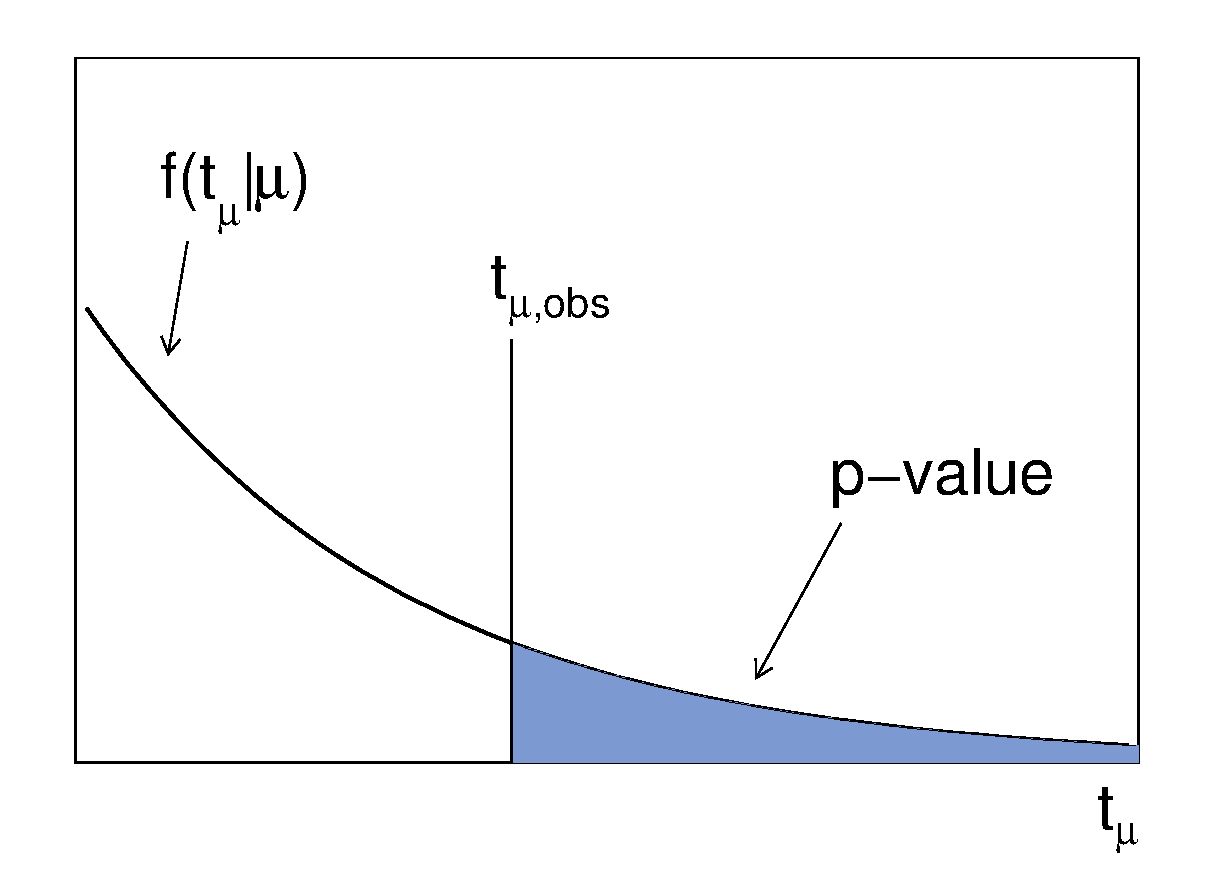
\includegraphics[width=0.45\textwidth]{stop/stat/Pval_tmu}}\hspace{0.05\textwidth}
					\subbottom[]{
						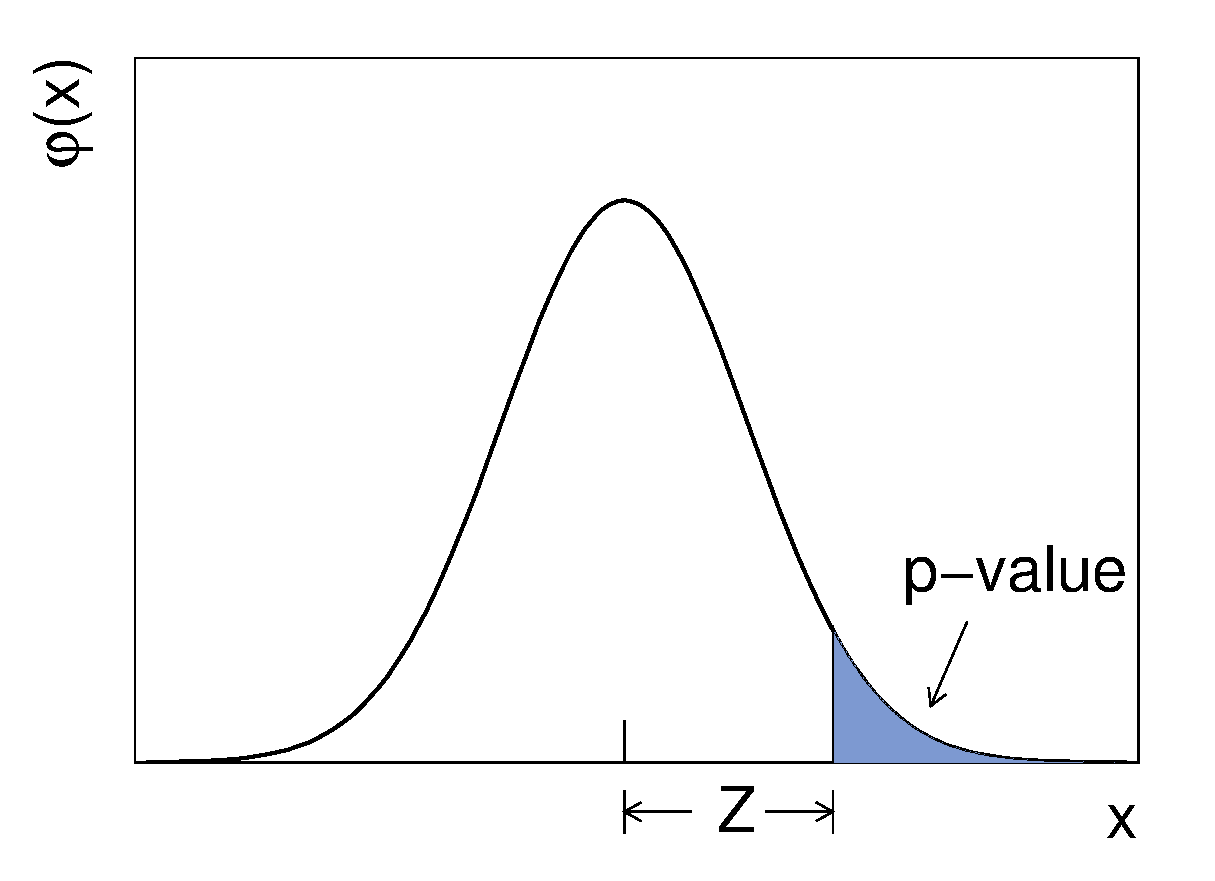
\includegraphics[width=0.45\textwidth]{stop/stat/Significance}}\hspace{0.05\textwidth}
				\caption{Illustration of the relation between the $p$-value obtained from an observed value of the test statistic $t_{\mu}$~(a), and the standard normal distribution showing the relation between the significance $Z$ and the $p$-value (taken from~\cite{Cowan:2010js}).}
				\label{fig:pval-sig}
			\end{figure}

			\noindent where, as shown in Figure~\ref{fig:pval-sig}~(a), $f(t)$ is integrated from the observed value of the test statistic, $t_{\mu,\mathrm{obs}}$, to infinity. In fact, a quantity which is equivalent to the $p$-value, the significance, $Z$, is instead considered. For convenience, the $p$-value is converted into the significance, $Z$, defined as the number of standard deviations $\sigma$ from the mean of a Gaussian distribution for which the integral of the tail of the curve is equal to $p$: 

			\begin{equation}
				Z = \Phi^{-1} \left ( 1 - p \right )
			\label{eq:Z_pval}
			\end{equation}

			\noindent Here, $\Phi^{-1}$ is the inverse of the cumulative distribution of the Gaussian, as it can be seen from Figure~\ref{fig:pval-sig}~(b). The particle physics community has chosen $Z = 5$ ($Z=3$) as the minimum value of significance needed to claim a discovery (evidence) against the background-only hypothesis. Such value of significance correspond to a $p$-value of $2.87 \times 10^{-7}$ and $p = 0.0013$, respectively. A significance of $1.64\sigma$ ($p = 0.05$) is instead used to exclude a given signal model.

			The choice of an appropriate test $t$ is an important step in the statistical hypothesis testing procedure. From Equation~\ref{eq:likelihood} a statistic test can be obtained as it follows: 

			\begin{equation}
				\lambda \left ( \mu_{\mathrm{s}} \right ) = \frac{L\left ( \mu_{\mathrm{s}}, \hat{\hat{\bm{\theta}}} \right )}{L\left ( \hat{\mu_{\mathrm{s}}}, \hat{\bm{\theta}} \right )}
			\label{eq:PLR}
			\end{equation}

			\noindent where the vector $\bm{\theta}$ takes into account the background normalisation factors and the nuisance parameters related to the systematic uncertainties. The numerator $L\left ( \mu_{\mathrm{s}}, \hat{\hat{\bm{\theta}}} \right )$ is the maximum for a given value of $\mu_{\mathrm{s}}$, while the denominator $L\left ( \hat{\mu_{\mathrm{s}}}, \hat{\bm{\theta}} \right )$ corresponds to the absolute maximum of the likelihood function. As shown in Equation~\ref{eq:PLR}, $0 < \lambda < 1$: the larger the values the better the agreement of the data with the hypothesis being tested. It is possible to define a test statistic, with the range required by the definition of the $p$-value in Equation~\ref{eq:pvalue}, as $t_{\mu,\mathrm{obs}} = -2 \ln \lambda \left ( \mu \right )$, where the larger the values the lower the compatibility between the observed data and the hypothesis being tested. Two test statistics can be defined, one for discovery and one for exclusion.

			The discovery of a new signal is targeted by testing the background only hypothesis, and in particular by using a \ac{PLR} function with $\mu_s = 0$, with the following definition:
			 % the former tests the background-only hypothesis and employs a \ac{PLR} function with $\mu_{\mathrm{s}} = 0$; the test can be defined as:
			\begin{align}
			\label{eq:test_discovery}
				\begin{split}
					q_0 & = 
					\begin{cases}
						-2 \ln \lambda \left( 0 \right ) & \hat{\mu_{\mathrm{s}}} \geq 0 \\
						0   & \hat{\mu_{\mathrm{s}}} < 0
					\end{cases}
				\end{split}
			\end{align}
			\noindent The test statistic $q_0$ is set to $0$ for negative $\hat{\mu_{\mathrm{s}}}$ such that the exclusion of the background-only hypothesis, when a deficit of events is observed in the \acp{SR}, can be avoided. 

			The exclusion of a signal model employs a test statistic defined as follows:
			\begin{align}
			\label{eq:test_exclusion}
				\begin{split}
					q_{\mu} & = 
					\begin{cases}
						-2 \ln \lambda \left( \mu_{\mathrm{s}} \right ) & \hat{\mu_{\mathrm{s}}} \leq \mu_{\mathrm{s}} \\
						0   & \hat{\mu_{\mathrm{s}}} > \mu_{\mathrm{s}}
					\end{cases}
				\end{split}
			\end{align}
			\noindent Here, a non-zero signal strength $\mu_s$ is assumed in the null hypothesis.

			% \begin{description}
			% 	\item [Discovery:] the background-only hypothesis is tested in this case; a \ac{PLR} function with $\mu_{\mathrm{s}} = 0$ is employed, and it can be defined as:
			% 	\begin{align}
			% 	\label{eq:test_discovery}
			% 		\begin{split}
			% 			q_0 & = 
			% 			\begin{cases}
			% 				-2 \ln \lambda \left( 0 \right ) & \hat{\mu_{\mathrm{s}}} \geq 0 \\
			% 				0   & \hat{\mu_{\mathrm{s}}} < 0
			% 			\end{cases}
			% 		\end{split}
			% 	\end{align}
			% 	\noindent here, $q_0$ is set to $0$ for negative $\hat{\mu_{\mathrm{s}}}$ such that the exclusion of the background-only hypothesis, when a deficit of events is observed in the \acp{SR}, can be avoided.

			% 	\item [Exclusion:] for the exclusion of a signal model, the test statistic can be defined as:
			% 	\begin{align}
			% 	\label{eq:test_exclusion}
			% 		\begin{split}
			% 			q_{\mu} & = 
			% 			\begin{cases}
			% 				-2 \ln \lambda \left( \mu_{\mathrm{s}} \right ) & \hat{\mu_{\mathrm{s}}} \leq \mu_{\mathrm{s}} \\
			% 				0   & \hat{\mu_{\mathrm{s}}} > \mu_{\mathrm{s}}
			% 			\end{cases}
			% 		\end{split}
			% 	\end{align}
			% 	\noindent here, the signal strength, $\mu_{\mathrm{s}}$, assumed to be non-zero in the null hypothesis.  
			% \end{description}

			Unfortunately, for signal models to which the analysis is poorly sensitive, Equation~\ref{eq:test_exclusion} can return a non-negligible probability and, although it can be argued that any constraint on such models should not be put, it is still possible that in the signal-plus-background hypothesis low $p$-values can be obtained when the observed events in the \acp{SR} are fewer than the predicted ones. The introduction of an alternative \acl{FoM} (FoM) for the exclusion can be employed~\cite{Read:2002hq}:

			\begin{equation}
				\mathrm{CL}_s = \frac{p_{\mu_{\mathrm{s}}}} {1 - p_{_\mathrm{b}}}
			\label{eq:cls}
			\end{equation}

			\noindent where $p_{_\mathrm{b}}$ and $p_{\mu_{\mathrm{s}}}$ correspond to the $p$-values of the background-only and signal-plus-background hypotheses, respectively. A $95\%$ \ac{CL} is reached when $\mathrm{CL}_s < 0.05$, \ie\ a threshold of $Z = 2$. Ultimately, when discovery and exclusion test statistics show similar distributions, this will translate into a numerator and denominator of the same order (Equation~\ref{eq:cls}), which guarantees that signals are not excluded, as one would expect.


			\subsection{Discovery and exclusion}

				The parameter estimation discussed in Section~\ref{sec:stat_ana} is the heart of the estimation of the \ac{SM}-background normalisation factors, which is an essential part of the background estimation procedure discussed in Section~\ref{sec:bkgest}. All the various \ac{CR} selections are plugged in a likelihood function of the form of Equation~\ref{eq:likelihood} which is then maximised in order to determine all the normalisation factors, nuisance parameters, and correlations between them. The so-obtained parameters are then used in Equation~\ref{eq:nevt_regionR}. 

				The statistical hypothesis testing procedure discussed in Section~\ref{sec:stat_ana} is used to evaluate the $p$-value for the background-only hypothesis to interpret the results in all the \acp{SR}. The likelihood function, including all the \acp{CR} and the \ac{SR} being tested, is employed to build a \ac{PLR} function. The yield predictions in such \ac{SR} are then determined solely by looking at the \ac{SM} processes \ie\ the signal strength, $\mu_{\mathrm{s}}$, is set to $0$. The Equation~\ref{eq:test_discovery} is then used to compute the $p$-value and the significance $Z$.%, using either toys the relevant asymptotic formula ~\cite{Cowan2011}.

				Finally, if no excess is observed in any of the \acp{SR}, the $\mathrm{CL}_s$ method is used to set exclusion limits on several signal hypotheses by computing the $q_0$ and $q_{\mathrm{\mu}}$ test statistics under the background-only hypothesis for a given signal strength, employing the minimisation of various likelihood functions. %For such reason, as already anticipated the \texttt{HistFitter} framework is employed~\cite{histfitter}.



	\section{Results and Interpretation}
	\label{sec:results}

		In this section the results of this analysis will be presented. The results of the background-only fit and the unblinded \acp{SR}, together with the relevant distributions, will be discussed in Section~\ref{subsec:bkgonly_fit} and~\ref{subsec:unblinded_SR}, respectively. Finally, in Section~\ref{subsec:limitset} the limits on different signal models will be presented, if no evidence for new physics is found.

 		\subsection{Background-only fit}
 		\label{subsec:bkgonly_fit}

 			The accuracy of the background estimation strategy, discussed in Chapter~\ref{ch:bkgest} is verified through dedicated sets of \acp{VR}. As previously anticipated, in such regions the data are expected to match the \ac{SM} predictions within the uncertainties, as the signal contamination is expected to be low. Figure~\ref{fig:extrapolation} shows where the VRs should generally lay such that the impact of any potential bias that may affect the \acp{TF} can be assessed. Before unblinding the data in the \acp{SR}, the necessary condition to be checked is the agreement between data and predictions in the \acp{VR}. Then the signal, if any, will be expected to appear in the \acp{SR} as an excess of events with respect to the background-only hypothesis, with no corresponding effect in the \acp{VR}. In the case of a background-only fit, a likelihood fit is performed only using the various \acp{CR} described in Section~\ref{subsec:crs} and Appendix~\ref{app:sumbkgest}. Figure~\ref{fig:CRs} shows the comparison between observed data and \ac{MC} predictions of all relevant variables in the \acp{CR}.
		
			\begin{figure}[!htb]
			  \centering
		    \subbottom[]{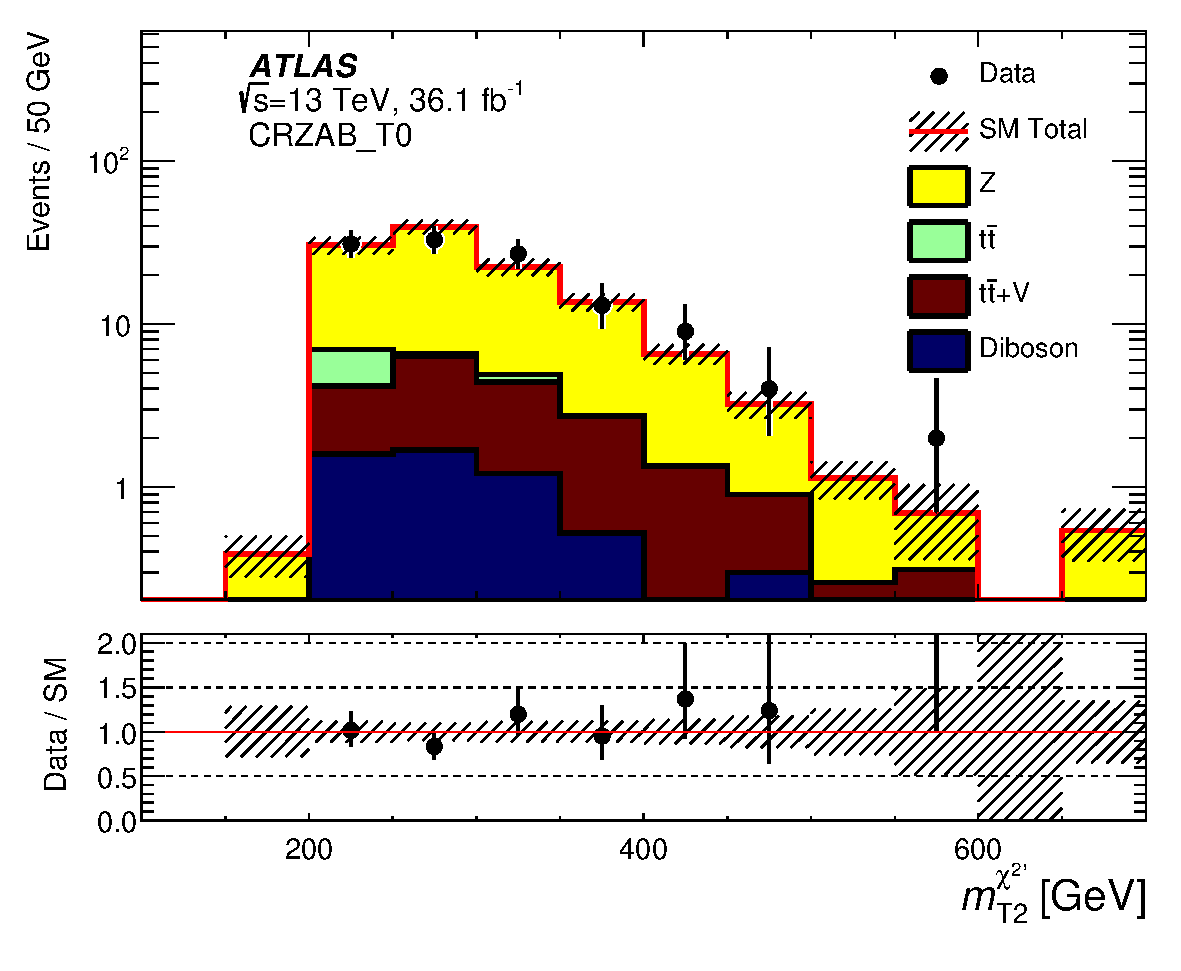
\includegraphics[width=0.48\textwidth]{figures/stop/CRs/Znunu/MT2Chi2Lep_CRZAB_T0_log}}
		    % \subbottom[]{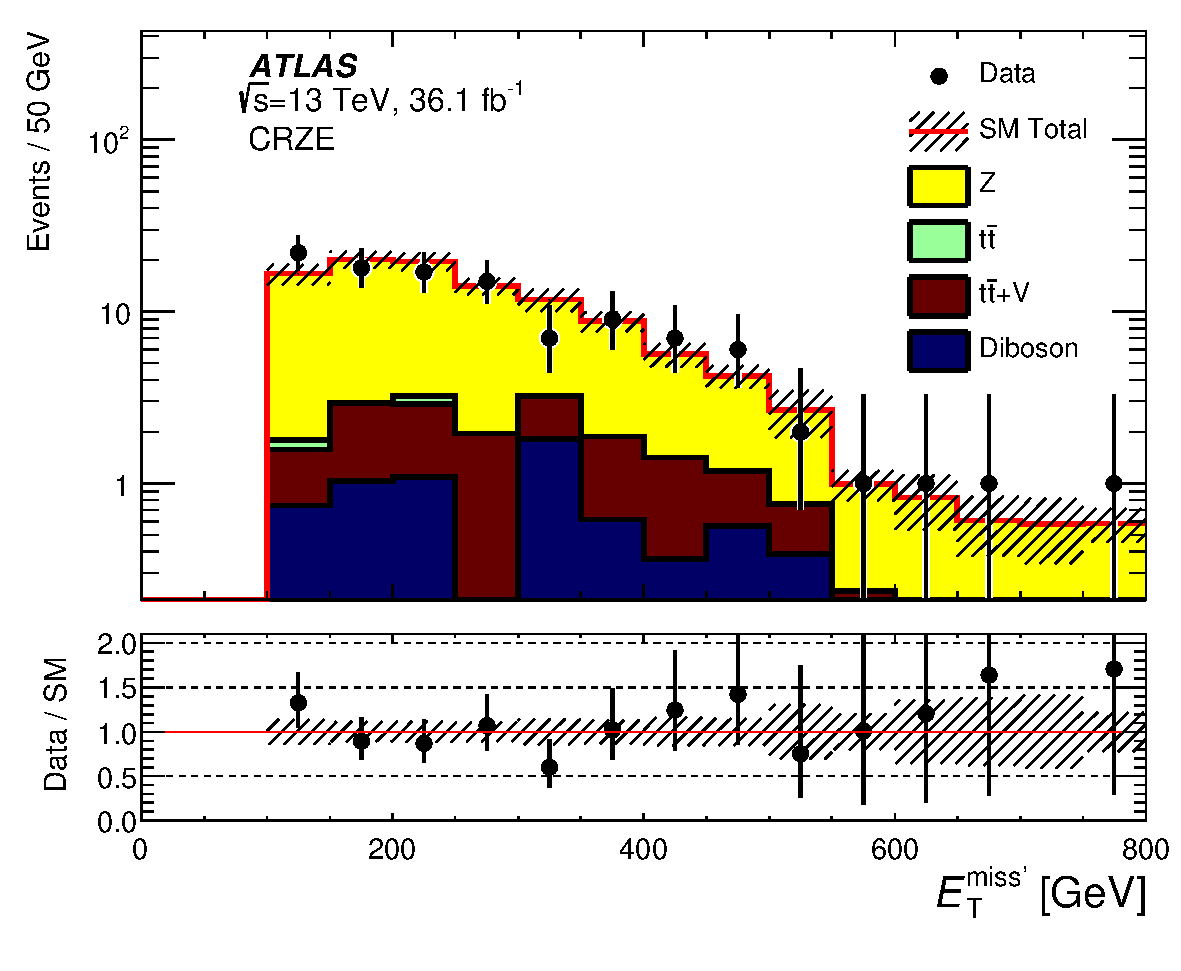
\includegraphics[width=0.48\textwidth]{figures/stop/CRs/Znunu/MetLep_CRZE_log}}
		    \subbottom[]{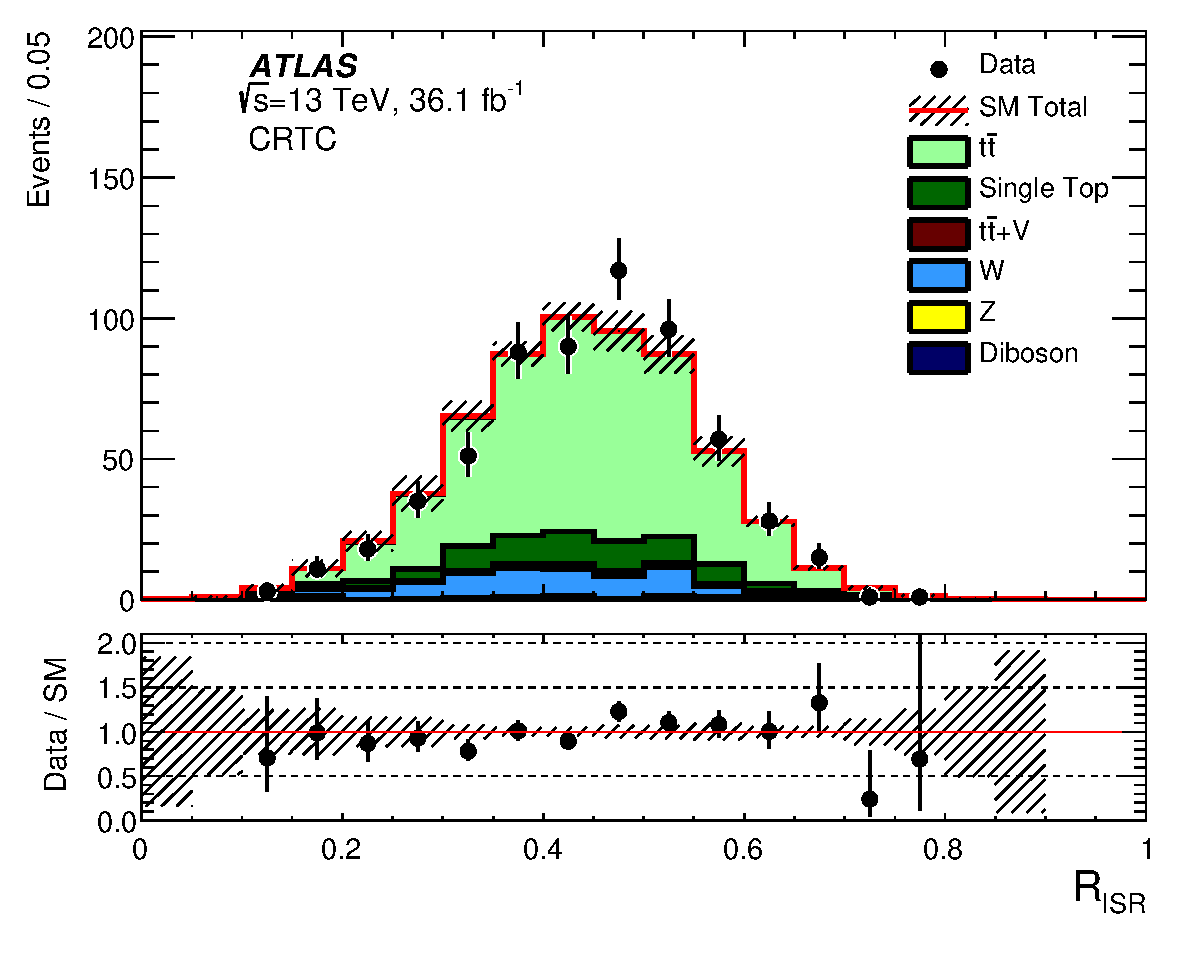
\includegraphics[width=0.48\textwidth]{figures/stop/CRs/ttbar/CA_RISR_CRTopC}}\\
		    \subbottom[]{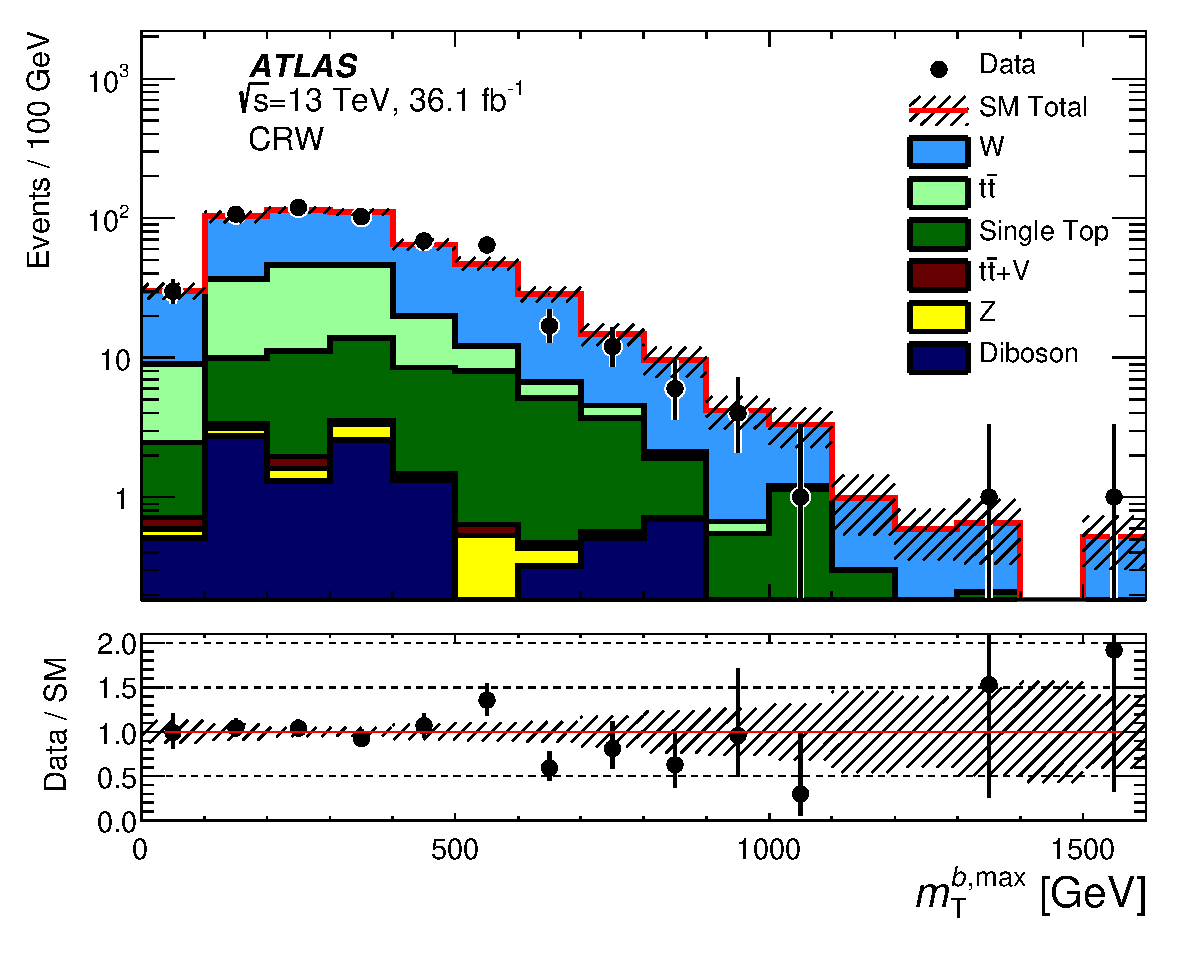
\includegraphics[width=0.48\textwidth]{figures/stop/CRs/Wjets/MtBMax_CRW_log}}
		    \subbottom[]{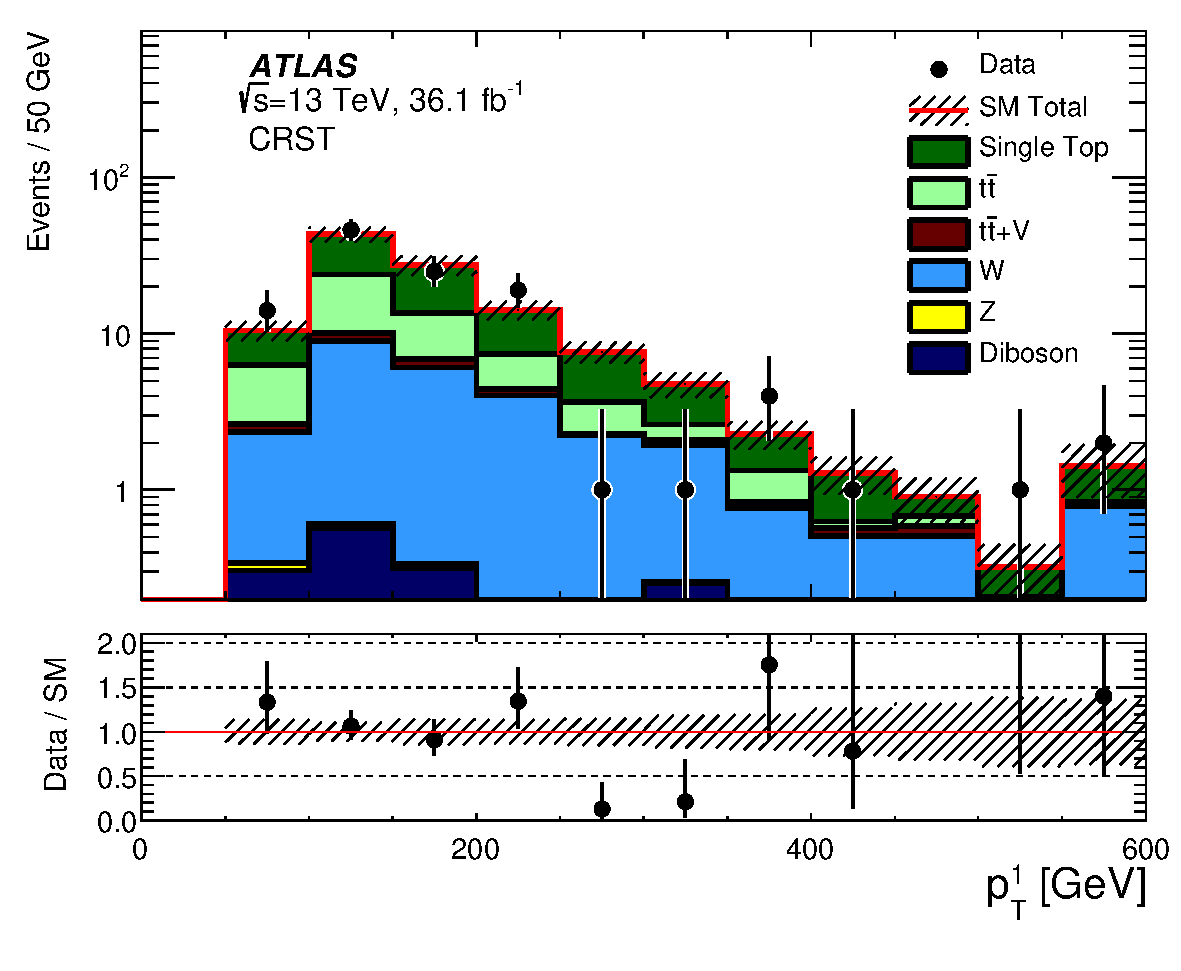
\includegraphics[width=0.48\textwidth]{figures/stop/CRs/singleTop/JetPt_1__CRST_log}}
		    \caption{Distributions of the most relevant variables: (a)~\mttwoprime\ in CRZAB-T0, (b)~\metprime\ in CRZE, (c)~\rISR\ in CRTC, (d)~\mtbmax\ in CRW, (e)~the transverse momentum of the second-leading-\pT\ jet in CRST. The stacked histograms show the \ac{SM} prediction, normalised using scale factors derived from the simultaneous fit to all backgrounds, discussed in Section~\ref{sec:stat_ana}. The ratio of data events to the total \ac{SM} prediction is also shown. The uncertainty band around the \ac{SM} prediction and in the ratio plot illustrates the combination of \ac{MC} statistical and detector-related systematic uncertainties. The rightmost bin includes overflow events~\cite{stop0L}.}
		    \label{fig:CRs}
			\end{figure}

			The result of the simultaneous fit procedure, described in Section~\ref{sec:stat_ana}, performed for each \ac{VR} is shown in Figure~\ref{fig:VRs}, which displays the agreement between data and \ac{MC} predictions. Here, the normalisation factors of the various \ac{SM} background estimation - all between $0.9 - 1.3$ - were used. Additionally, in all the \acp{VR} the signal contamination was checked for all the signals considered that have not yet been excluded. The largest signal contamination is $\sim 25\%$ in the VRTs for top-squark masses below $350$ \GeV\ and in VRZD and VRZE near top-squark masses of $700$ \GeV.

			\begin{figure}[!htb]
			  \begin{center}
			    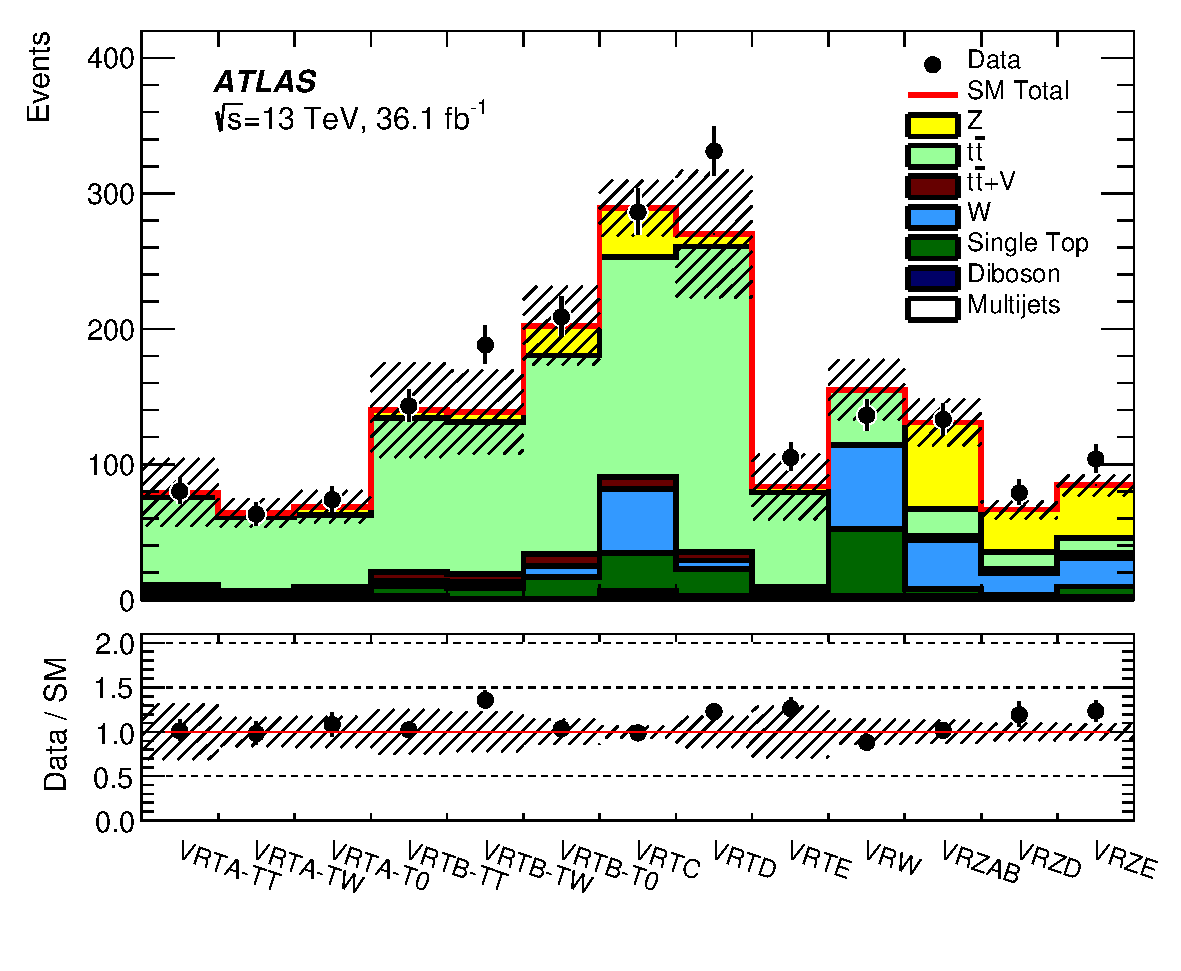
\includegraphics[width=.8\textwidth]{figures/stop/regionSummaryVR}
			    \caption{Yields for all the \acp{VR} after the likelihood fit. The stacked histograms show the \ac{SM} prediction and the uncertainty band around the \ac{SM} prediction shows the total uncertainty, which consists of the \ac{MC} statistical uncertainties, detector-related systematic uncertainties, and theoretical uncertainties in the extrapolation from \ac{CR} to \ac{VR}.} 
			    \label{fig:VRs}
			  \end{center}
			\end{figure}


 		\subsection{Opening Pandora's box: unblinded \acp{SR}}
 		\label{subsec:unblinded_SR}

 			The good agreement found in the \acp{CR} and \acp{VR} gives confidence in the modelling of the relevant \ac{SM} backgrounds and their estimation, therefore the \acp{SR} can now be unblinded. The event data counts are compared to the expected total number of background events in Tables~\ref{tab:srABYields},~\ref{tab:srCYields}, and~\ref{tab:srDEYields}. Figure~\ref{fig:srSummary} shows a summary of all the \ac{SR} yields after having performed the simultaneous likelihood fit.	
			
			\begin{table}[htpb]
				\caption{Observed and expected yields, before and after the fit, for SRA and SRB. The uncertainties include MC statistical uncertainties, detector-related systematic uncertainties, and theoretical uncertainties in the extrapolation from CR to SR~\cite{stop0L}.}
			  \begin{center}
					{\renewcommand{\arraystretch}{1.2}
					\begin{tabular}{lcccccc}
\toprule
 & {\textbf{SRA-TT}} & {\textbf{SRA-TW}} & {\textbf{SRA-T0}} & {\textbf{SRB-TT}} & {\textbf{SRB-TW}} & {\textbf{SRB-T0}}\\ \midrule 
{\textbf{Observed}} & {$11$} & {$9$} & {$18$} & {$38$} & {$53$} & {$206$} \\ \midrule 
{\textbf{Total SM (fit)}} & \multicolumn{1}{c}{$8.6\phantom{0} \pm 2.1\phantom{0}$} & \multicolumn{1}{c}{$9.3\phantom{0} \pm 2.2\phantom{0}$} & \multicolumn{1}{c}{$18.7\phantom{0} \pm 2.7\phantom{0}$} & \multicolumn{1}{c}{$39.3\phantom{0} \pm 7.6\phantom{0}$} & \multicolumn{1}{c}{$52.4\phantom{0} \pm 7.4\phantom{0}$} & \multicolumn{1}{c}{$179\phantom{000} \pm 26\phantom{000}$}\\ \midrule 
{\ttbar} & \multicolumn{1}{c}{$0.71\;_{-\;0.71}^{+\;0.91}$} & \multicolumn{1}{c}{$0.51\;_{-\;0.51}^{+\;0.55}$} & \multicolumn{1}{c}{$\phantom{1}1.31 \pm 0.64$} & \multicolumn{1}{c}{$\phantom{3}7.3\phantom{0} \pm 4.3\phantom{0}$} & \multicolumn{1}{c}{$12.4\phantom{0} \pm 5.9\phantom{0}$} & \multicolumn{1}{c}{$\phantom{1}43\phantom{000} \pm 22\phantom{000}$}\\ 
{\Wjets} & \multicolumn{1}{c}{$0.82 \pm 0.15$} & \multicolumn{1}{c}{$0.89 \pm 0.56$} & \multicolumn{1}{c}{$\phantom{1}2.00 \pm 0.83$} & \multicolumn{1}{c}{$\phantom{3}7.8\phantom{0} \pm 2.8\phantom{0}$} & \multicolumn{1}{c}{$\phantom{5}4.8\phantom{0} \pm 1.2\phantom{0}$} & \multicolumn{1}{c}{$\phantom{1}25.8\phantom{0} \pm \phantom{2}8.8\phantom{0}$}\\ 
{\Zjets} & \multicolumn{1}{c}{$2.5\phantom{0} \pm 1.3\phantom{0}$} & \multicolumn{1}{c}{$4.9\phantom{0} \pm 1.9\phantom{0}$} & \multicolumn{1}{c}{$\phantom{1}9.8\phantom{0} \pm 1.6\phantom{0}$} & \multicolumn{1}{c}{$\phantom{3}9.0\phantom{0} \pm 2.8\phantom{0}$} & \multicolumn{1}{c}{$16.8\phantom{0} \pm 4.1\phantom{0}$} & \multicolumn{1}{c}{$\phantom{1}60.7\phantom{0} \pm \phantom{2}9.6\phantom{0}$}\\ 
{\ttV} & \multicolumn{1}{c}{$3.16 \pm 0.66$} & \multicolumn{1}{c}{$1.84 \pm 0.39$} & \multicolumn{1}{c}{$\phantom{1}2.60 \pm 0.53$} & \multicolumn{1}{c}{$\phantom{3}9.3\phantom{0} \pm 1.7\phantom{0}$} & \multicolumn{1}{c}{$10.8\phantom{0} \pm 1.6\phantom{0}$} & \multicolumn{1}{c}{$\phantom{1}20.5\phantom{0} \pm \phantom{2}3.2\phantom{0}$}\\ 
{Single top} & \multicolumn{1}{c}{$1.20 \pm 0.81$} & \multicolumn{1}{c}{$0.70 \pm 0.42$} & \multicolumn{1}{c}{$\phantom{1}2.9\phantom{0} \pm 1.5\phantom{0}$} & \multicolumn{1}{c}{$\phantom{3}4.2\phantom{0} \pm 2.2\phantom{0}$} & \multicolumn{1}{c}{$\phantom{5}5.9\phantom{0} \pm 2.8\phantom{0}$} & \multicolumn{1}{c}{$\phantom{1}26\phantom{000} \pm 13\phantom{000}$}\\ 
{Dibosons} & \multicolumn{1}{c}{${-} {-}$} & \multicolumn{1}{c}{$0.35 \pm 0.26$} & \multicolumn{1}{c}{${-} {-}$} & \multicolumn{1}{c}{$\phantom{3}0.13 \pm 0.07$} & \multicolumn{1}{c}{$\phantom{5}0.60 \pm 0.43$} & \multicolumn{1}{c}{$\phantom{17}1.04 \pm \phantom{2}0.73$}\\ 
{Multijets} & \multicolumn{1}{c}{$0.21 \pm 0.10$} & \multicolumn{1}{c}{$0.14 \pm 0.09$} & \multicolumn{1}{c}{$\phantom{1}0.12 \pm 0.07$} & \multicolumn{1}{c}{$\phantom{3}1.54 \pm 0.64$} & \multicolumn{1}{c}{$\phantom{5}1.01 \pm 0.88$} & \multicolumn{1}{c}{$\phantom{17}1.8\phantom{0} \pm \phantom{2}1.5\phantom{0}$}\\ \midrule 
{\textbf{Total SM (exp)}} & \multicolumn{1}{c}{$7.1\phantom{3}\phantom{3}$}  & \multicolumn{1}{c}{$7.9\phantom{3}\phantom{3}$}  & \multicolumn{1}{c}{$16.3\phantom{3}\phantom{3}$}  & \multicolumn{1}{c}{$32.4\phantom{3}\phantom{3}$}  & \multicolumn{1}{c}{$46.1\phantom{3}\phantom{3}$}  & \multicolumn{1}{c}{$162\phantom{3}\phantom{2}$} \\  
\bottomrule
\end{tabular}

					}
				\end{center}
				\label{tab:srABYields}
			\end{table}

			\begin{table}[htpb]
			  \caption{Observed and expected yields, before and after the fit.
			The uncertainties include MC statistical uncertainties, detector-related systematic uncertainties, and theoretical uncertainties in the extrapolation from CR to SR~\cite{stop0L}.}
			  \begin{center}
			{\renewcommand{\arraystretch}{1.2}
			\begin{tabular}{lccccc}
\toprule
& {\textbf{SRC1}} & {\textbf{SRC2}} & {\textbf{SRC3}} & {\textbf{SRC4}} & {\textbf{SRC5}}\\ \midrule 
{\textbf{Observed}} & \multicolumn{1}{c}{$20$} & \multicolumn{1}{c}{$22$} & \multicolumn{1}{c}{$22$} & \multicolumn{1}{c}{$1$} & \multicolumn{1}{c}{$0$} \\ \midrule
{\textbf{Total SM (fit)}} & {$20.6\phantom{0} \pm 6.5\phantom{0}$} & {$27.6\phantom{0} \pm 4.9\phantom{0}$} & {$18.9\phantom{0} \pm 3.4\phantom{0}$} & {$7.7\phantom{0} \pm 1.2\phantom{0}$} & {$0.91 \pm 0.73$}\\ \midrule 
{\ttbar} & 	{$12.9\phantom{0} \pm 5.9\phantom{0}$} & \multicolumn{1}{c}{$22.1\phantom{0} \pm 4.3\phantom{0}$} & \multicolumn{1}{c}{$14.6\phantom{0} \pm 3.2\phantom{0}$} & \multicolumn{1}{c}{$4.91 \pm 0.97$} & \multicolumn{1}{c}{$0.63\;_{-\;0.63}^{+\;0.70}$}\\ 
{\Wjets} & \multicolumn{1}{c}{$\phantom{2}0.80 \pm 0.37$} & \multicolumn{1}{c}{$\phantom{2}1.93 \pm 0.49$} & \multicolumn{1}{c}{$\phantom{1}1.91 \pm 0.62$} & \multicolumn{1}{c}{$1.93 \pm 0.46$} & \multicolumn{1}{c}{$0.21 \pm 0.12$}\\ 
{\Zjets} & \multicolumn{1}{c}{${-} {-}$} & \multicolumn{1}{c}{${-} {-}$} & \multicolumn{1}{c}{${-} {-}$} & \multicolumn{1}{c}{${-} {-}$} & \multicolumn{1}{c}{${-} {-}$}\\ 
{\ttV} & \multicolumn{1}{c}{$\phantom{2}0.29 \pm 0.16$} & \multicolumn{1}{c}{$\phantom{2}0.59 \pm 0.38$} & \multicolumn{1}{c}{$\phantom{1}0.56 \pm 0.31$} & \multicolumn{1}{c}{$0.08 \pm 0.08$} & \multicolumn{1}{c}{$0.06 \pm 0.02$}\\ 
{Single top} & \multicolumn{1}{c}{$\phantom{2}1.7\phantom{0} \pm 1.3\phantom{0}$} & \multicolumn{1}{c}{$\phantom{2}1.2\phantom{0}\;_{-\;1.2}^{+\;1.4\phantom{0}}$} & \multicolumn{1}{c}{$\phantom{1}1.22 \pm 0.69$} & \multicolumn{1}{c}{$0.72 \pm 0.37$} & \multicolumn{1}{c}{${-} {-}$}\\ 
{Dibosons} & \multicolumn{1}{c}{$\phantom{2}0.39 \pm 0.33$} & \multicolumn{1}{c}{$\phantom{2}0.21\;_{-\;0.21}^{+\;0.23}$} & \multicolumn{1}{c}{$\phantom{1}0.28 \pm 0.18$} & \multicolumn{1}{c}{${-} {-}$} & \multicolumn{1}{c}{${-} {-}$}\\ 
{Multijets} & \multicolumn{1}{c}{$\phantom{2}4.6\phantom{0} \pm 2.4\phantom{0}$} & \multicolumn{1}{c}{$\phantom{2}1.58 \pm 0.77$} & \multicolumn{1}{c}{$\phantom{1}0.32 \pm 0.17$} & \multicolumn{1}{c}{$0.04 \pm 0.02$} & \multicolumn{1}{c}{${-} {-}$}\\ \midrule
{\textbf{Total SM (exp)}} & \multicolumn{1}{c}{$25.4\phantom{3}\phantom{3}$}  & \multicolumn{1}{c}{$36.0\phantom{3}\phantom{3}$}  & \multicolumn{1}{c}{$24.2\phantom{3}\phantom{3}$}  & \multicolumn{1}{c}{$9.2\phantom{3}\phantom{3}$}  & \multicolumn{1}{c}{$1.1\phantom{3}\phantom{4}$} \\ 
\bottomrule
\end{tabular}

			}
			\end{center}
			\label{tab:srCYields}
			\end{table}

			\begin{table}[htpb]
			  \caption{Observed and expected yields, before and after the fit, for SRD and SRE.
			The uncertainties include MC statistical uncertainties, detector-related systematic uncertainties, and theoretical uncertainties in the extrapolation from CR to SR~\cite{stop0L}.}
			  \begin{center}
			{\renewcommand{\arraystretch}{1.2}
			\begin{tabular}{lccc}
\toprule
 & {\textbf{SRD-low}} & {\textbf{SRD-high}} & {\textbf{SRE}}\\ \midrule 
{\textbf{Observed}} & \multicolumn{1}{c}{$27$} & \multicolumn{1}{c}{$11$} & \multicolumn{1}{c}{$3$} \\ \midrule
{\textbf{Total SM (fit)}} & \multicolumn{1}{c}{$25.1\phantom{0} \pm 6.2\phantom{0}$} & \multicolumn{1}{c}{$8.5\phantom{0} \pm 1.5\phantom{0}$} & \multicolumn{1}{c}{$3.64 \pm 0.79$}\\ \midrule 
{\ttbar} & \multicolumn{1}{c}{$\phantom{2}3.3\phantom{0} \pm 3.3\phantom{0}$} & \multicolumn{1}{c}{$0.98 \pm 0.88$} & \multicolumn{1}{c}{$0.21\;_{-\;0.21}^{+\;0.39}$}\\ 
{\Wjets} & \multicolumn{1}{c}{$\phantom{2}6.1\phantom{0} \pm 2.9\phantom{0}$} & \multicolumn{1}{c}{$1.06 \pm 0.34$} & \multicolumn{1}{c}{$0.52 \pm 0.27$}\\ 
{\Zjets} & \multicolumn{1}{c}{$\phantom{2}6.9\phantom{0} \pm 1.5\phantom{0}$} & \multicolumn{1}{c}{$3.21 \pm 0.62$} & \multicolumn{1}{c}{$1.36 \pm 0.25$}\\ 
{\ttV} & \multicolumn{1}{c}{$\phantom{2}3.94 \pm 0.85$} & \multicolumn{1}{c}{$1.37 \pm 0.32$} & \multicolumn{1}{c}{$0.89 \pm 0.19$}\\ 
{Single top} & \multicolumn{1}{c}{$\phantom{2}3.8\phantom{0} \pm 2.1\phantom{0}$} & \multicolumn{1}{c}{$1.51 \pm 0.74$} & \multicolumn{1}{c}{$0.66 \pm 0.49$}\\ 
{Dibosons} & \multicolumn{1}{c}{${-} {-}$} & \multicolumn{1}{c}{${-} {-}$} & \multicolumn{1}{c}{${-} {-}$}\\ 
{Multijets} & \multicolumn{1}{c}{$\phantom{2}1.12 \pm 0.37$} & \multicolumn{1}{c}{$0.40 \pm 0.15$} & \multicolumn{1}{c}{${-} {-}$}\\ \midrule 
{\textbf{Total SM (exp.)}} & \multicolumn{1}{c}{$22.4\phantom{3}\phantom{3}$}  & \multicolumn{1}{c}{$7.7\phantom{3}\phantom{3}$}  & \multicolumn{1}{c}{$3.02\phantom{3}\phantom{4}$} \\ 
\midrule
\end{tabular}

			}
			\end{center}
			\label{tab:srDEYields}
			\end{table}

			The analysis yielded no significant excess above the \ac{SM} prediction in any of the \acp{SR}, as it can be seen in Figure~\ref{fig:srSummary}. The smallest $p$-values are $27\%$, $27\%$, and $29\%$ for SRB-T0, SRD-high, and SRA-TT, respectively. The largest deficit in the data is observed in SRC4 where only one event is observed against $7.7$ expected background events and this is probably due to the very low statistics.

			\begin{figure}[htpb]
			  \begin{center}
			    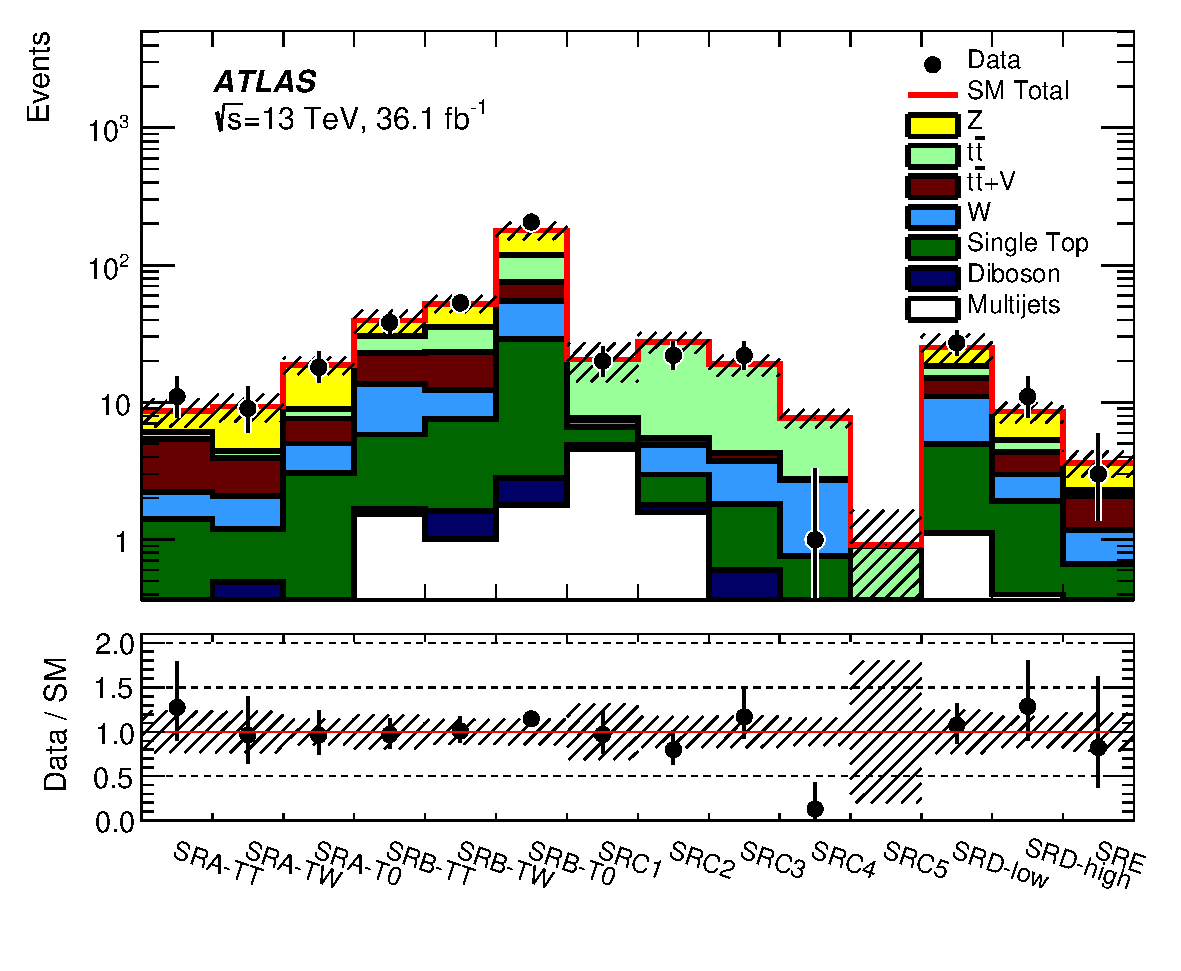
\includegraphics[width=0.8\textwidth]{stop/fit/regionSummaryLog}
			    \caption{Yields for all signal regions after the likelihood fit. The stacked histograms show the SM prediction and the hatched uncertainty band around the SM prediction shows total uncertainty, which consists of the MC statistical uncertainties, detector-related systematic uncertainties, and theoretical uncertainties in the extrapolation from CR to SR~\cite{stop0L}.} 
			    \label{fig:srSummary}
			  \end{center}
			\end{figure}

			Figure~\ref{fig:SRs} shows the $N-1$ distributions, obtained by applying all the \ac{SR} selections but the cut on the variable plotted, of \met, \mttwo, \mtbmax, \mt, \rISR, and \HT, for the various \acp{SR}, with \rISR\ being shown combining SRC1--5. The background predictions in these distributions are scaled to the values determined from the simultaneous fit. A good data-SM prediction agreement is observed across the whole kinematical range in the displayed plots, confirming once again the reliability of the presented background estimation strategy. 

			\begin{figure}[htpb]
			  \begin{center}
			    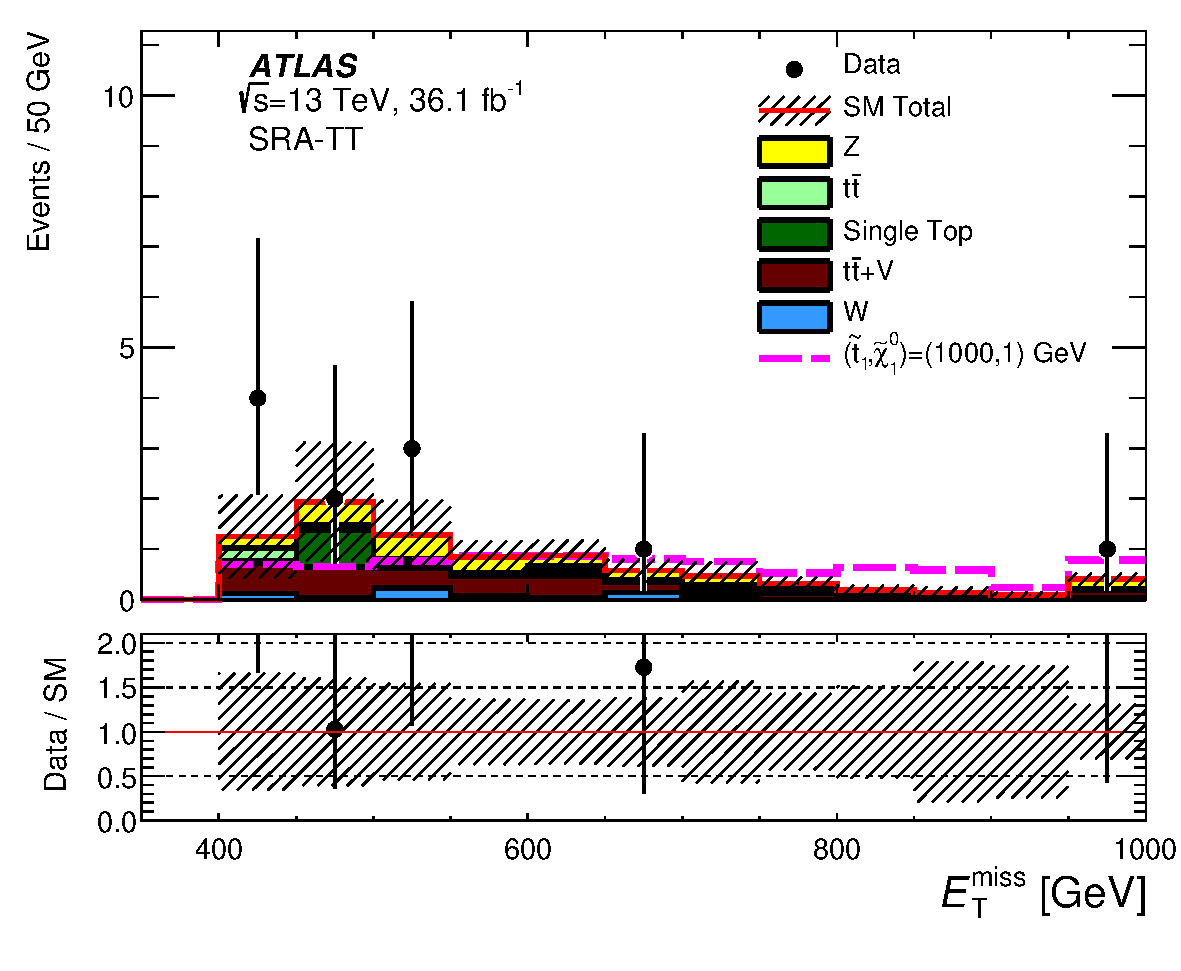
\includegraphics[width=0.49\textwidth]{stop/SRA/Met_SRA_TT}
			    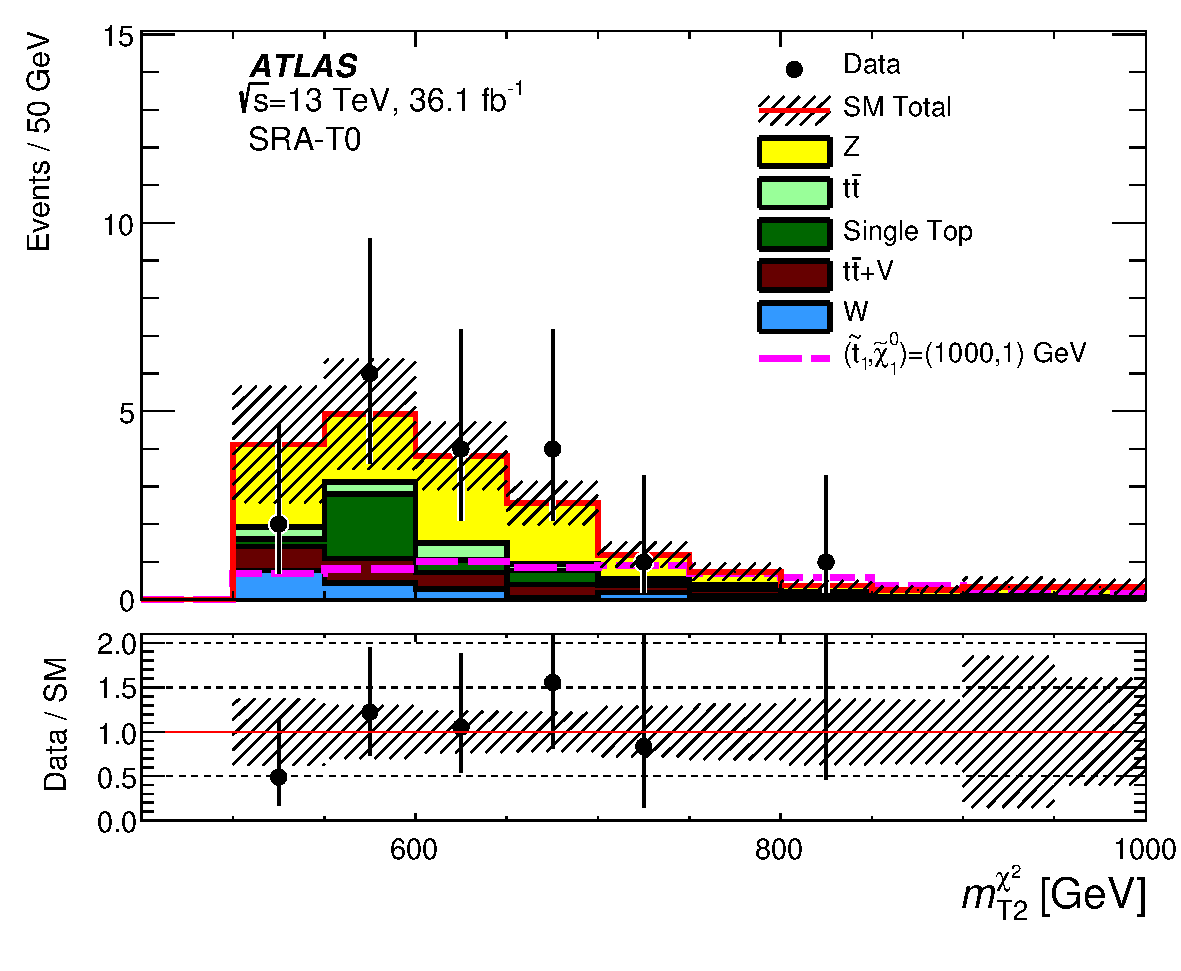
\includegraphics[width=0.49\textwidth]{stop/SRA/MT2Chi2_SRA_T0}\\%\hspace{0.05\textwidth}
			    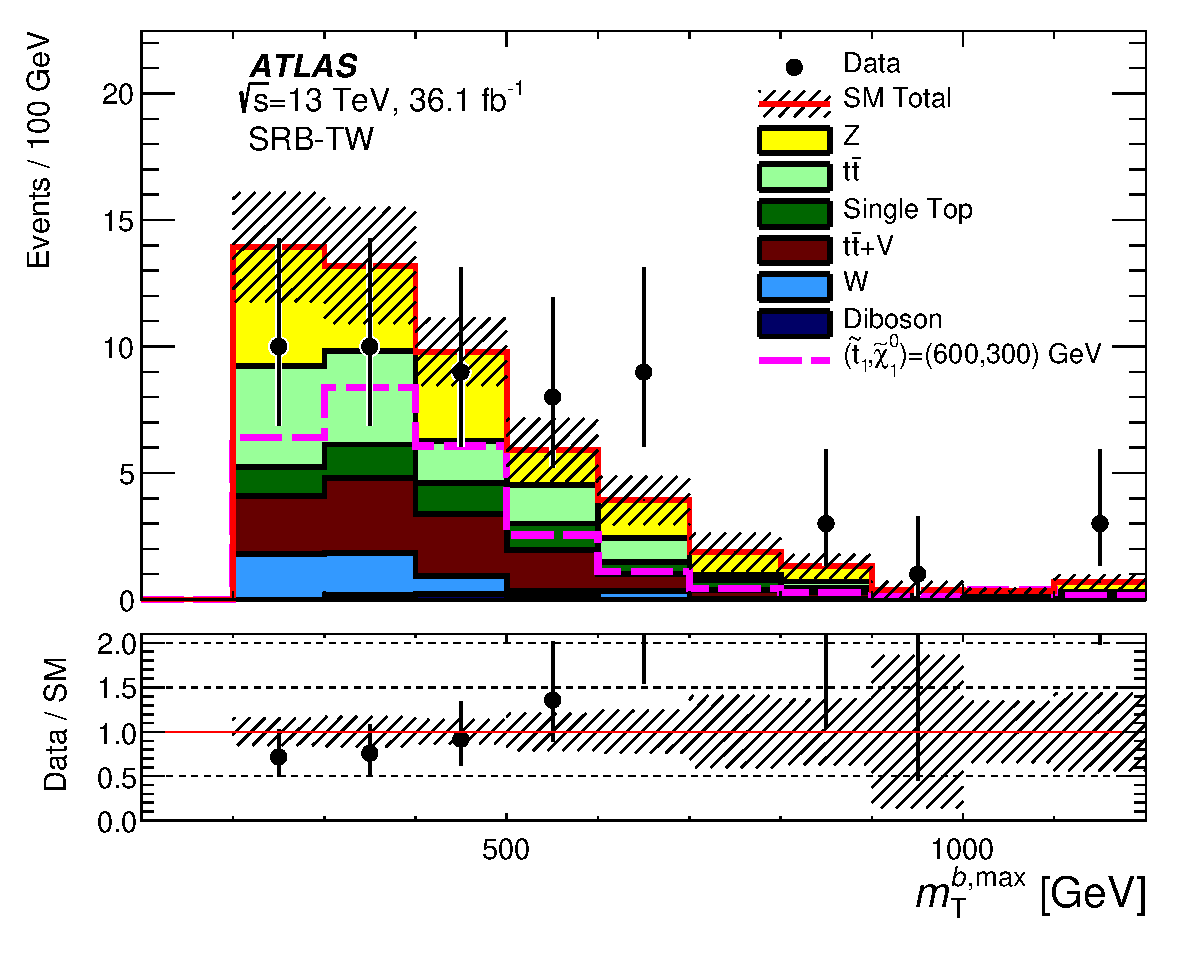
\includegraphics[width=0.49\textwidth]{stop/SRB/MtBMax_SRB_TW}
			    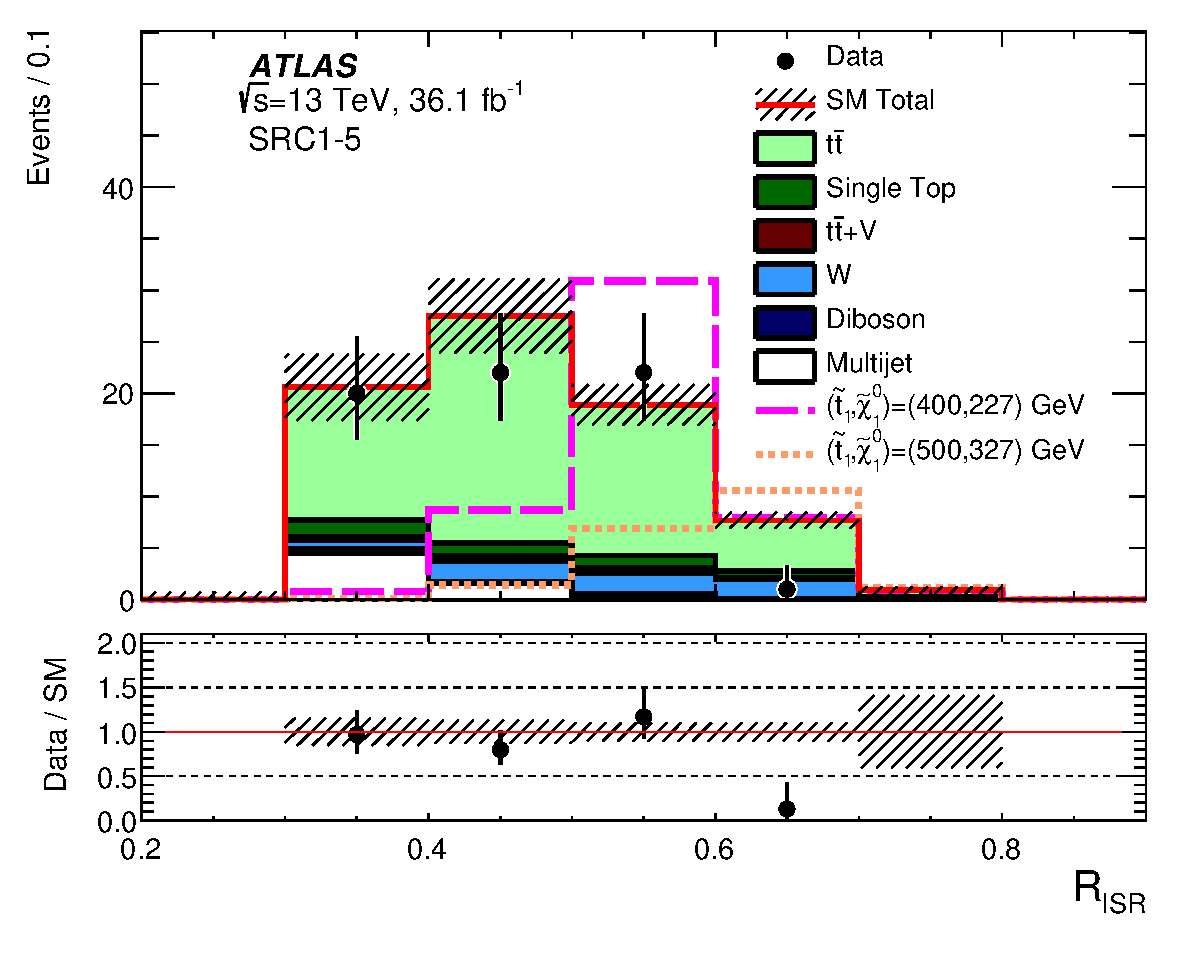
\includegraphics[width=0.49\textwidth]{stop/SRC/CA_RISR_SRC1_5}\\%\hspace{0.05\textwidth}
			    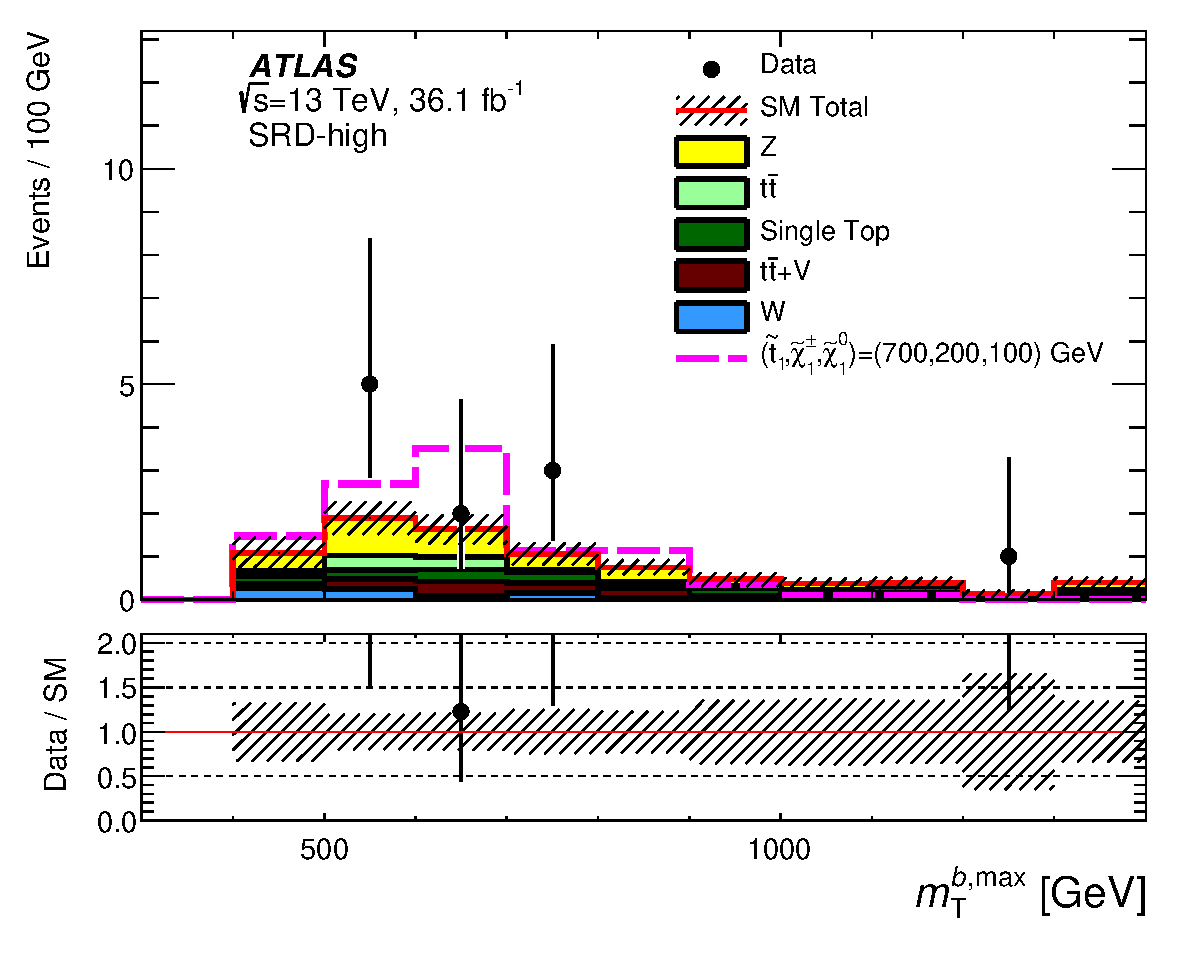
\includegraphics[width=0.49\textwidth]{stop/SRD/MtBMax_SRD_high}
			    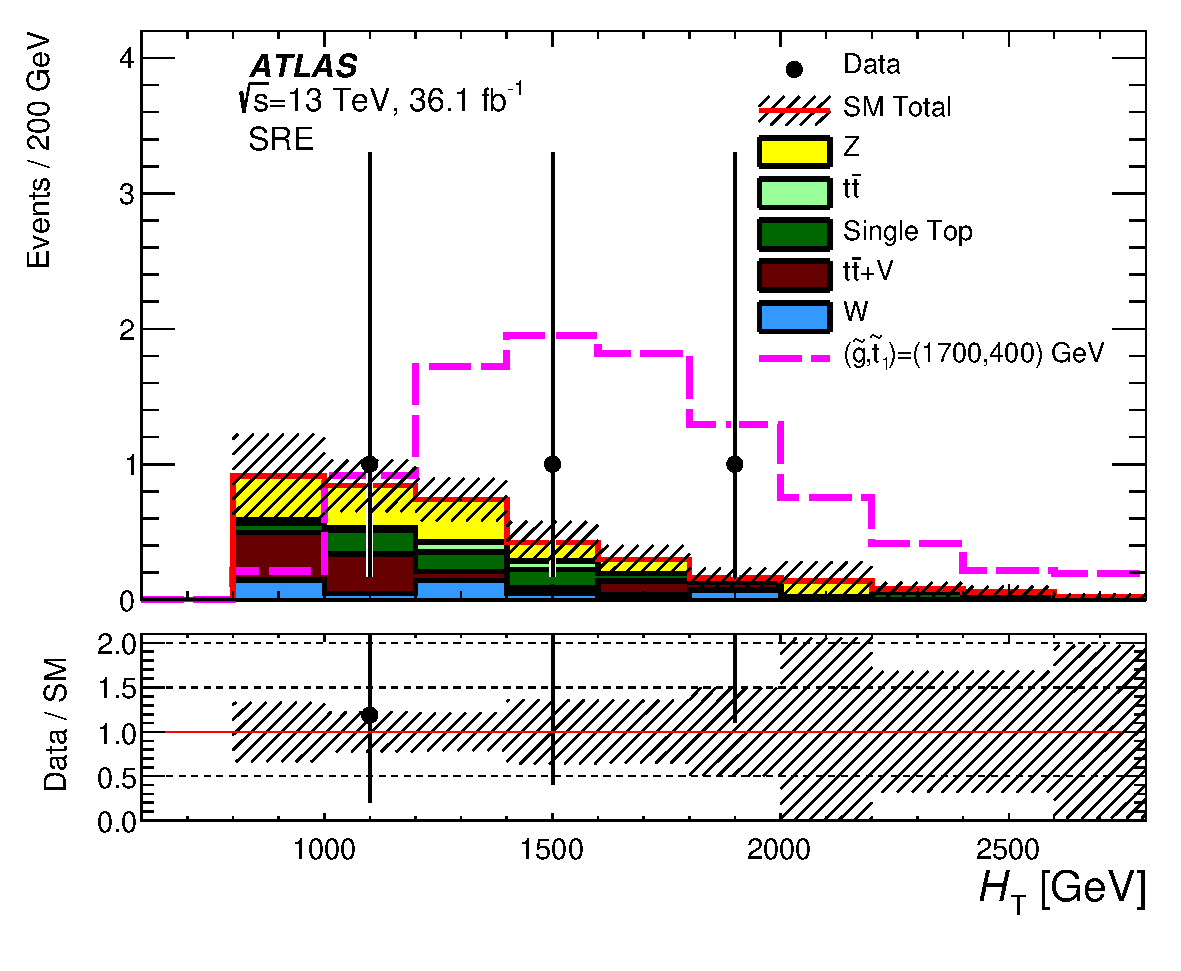
\includegraphics[width=0.49\textwidth]{stop/SRE/Ht_SRE}
			    \caption{Distributions of \met\ for SRA-TT, \mttwo\ for SRA-T0, \mtbmax\ for SRB-TW, \rISR\ for SRC1--5, \mtbmax\ for SRD-high and \HT\ for SRE obtained after having performed the likelihood fit. The stacked histograms show the SM prediction and the hatched uncertainty band around the SM prediction shows the MC statistical and detector-related systematic uncertainties. For each variable, the distribution for a representative signal point is shown~\cite{stop0L}.}
			    \label{fig:SRs}
			  \end{center}
			\end{figure}



 		\subsection{Setting the limits}
 		\label{subsec:limitset}

			As no excess over the \ac{SM} is observed in any of the investigated \acp{SR}, exclusion limits are set. In particular, the $\mathrm{CL}_s$ method, discussed in Section~\ref{sec:stat_ana}, is used to perform the exclusion fits. Model-independent limits on the visible \ac{BSM} cross section, defined as $\sigma_{\mathrm{vis}} = S^{95}_{\textnormal{obs}}/\int\!\!{\mathcal L}\,dt$, where $S^{95}_{\textnormal{obs}}$ is the 95\% CL upper limit on the number of signal events, are reported in Table~\ref{tab:upLimits}.

			\begin{table}[htpb]
				\caption{Left to right: 95\% CL upper limits on the average visible cross section ($\langle\sigma A \epsilon\rangle_{\mathrm obs}^{95}$) where the average comes from possibly multiple production channels and on the number of signal events ($S_{\mathrm obs}^{95}$ ).  The third column ($S_{\mathrm exp}^{95}$) shows the 95\% CL upper limit on the number of signal events, given the expected number (and $\pm 1\sigma$ excursions of the expected number) of background events. The discovery $p$-value ($p$) and the corresponding significance ($Z$) are shown in the last column~\cite{stop0L}.}
				\label{tab:upLimits}
				\begin{center}
		    	{\renewcommand{\arraystretch}{1.3}
\begin{tabular*}{\textwidth}{@{\extracolsep{\fill}}lccccc}
\noalign{\smallskip}\toprule\noalign{\smallskip}
{\textbf{Signal channel}}                        & $\langle{\mathrm{\sigma}} A \epsilon\rangle_{\mathrm{obs}}^{95}$ [fb]  &  $S_{\mathrm{obs}}^{95}$  & $S_{\mathrm{exp}}^{95}$ & $p$ ($Z$)  \\
\noalign{\smallskip}\midrule\noalign{\smallskip}

SRA-TT    & $0.30$ &  $11.0$ & $ { 8.7 }^{ +3.0 }_{ -1.4 }$ & $ 0.23$~$(0.74)$ \\%
SRA-TW    & $0.27$ &  $9.6$ & $ { 9.6 }^{ +2.8 }_{ -2.1 }$ & $ 0.50$~$(0.00)$ \\%
SRA-T0    & $0.31$ &  $11.2$ & $ { 11.5 }^{ +3.8 }_{ -2.0 }$ & $ 0.50$~$(0.00)$ \\%
SRB-TT    & $0.54$ &  $19.6$ & $ { 20.0 }^{ +6.5 }_{ -4.9 }$ & $ 0.50$~$(0.00)$ \\%
SRB-TW    & $0.60$ &  $21.7$ & $ { 21.0 }^{ +7.3 }_{ -4.3 }$ & $ 0.50$~$(0.00)$ \\%
SRB-T0    & $2.19$ &  $80$ & $ { 58 }^{ +23 }_{ -17 }$ & $ 0.13$~$(1.15)$ \\%
SRC1    & $0.42$ &  $15.1$ & $ { 15.8 }^{ +4.8 }_{ -3.5 }$ & $ 0.50$~$(0.00)$ \\%
SRC2    & $0.31$ &  $11.2$ & $ { 13.9 }^{ +5.9 }_{ -3.6 }$ & $ 0.50$~$(0.00)$ \\%
SRC3    & $0.42$ &  $15.3$ & $ { 12.3 }^{ +4.7 }_{ -3.4 }$ & $ 0.27$~$(0.62)$ \\%
SRC4    & $0.10$ &  $3.5$ & $ { 6.7 }^{ +2.8 }_{ -1.8 }$ & $ 0.50$~$(0.00)$ \\%
SRC5    & $0.09$ &  $3.2$ & $ { 3.0 }^{ +1.1 }_{ -0.1 }$ & $ 0.23$~$(0.74)$ \\%
SRD-low    & $0.50$ &  $17.9$ & $ { 16.4 }^{ +6.3 }_{ -4.0 }$ & $ 0.36$~$(0.35)$ \\%
SRD-high    & $0.30$ &  $10.9$ & $ { 8.0 }^{ +3.4 }_{ -1.3 }$ & $ 0.21$~$(0.79)$ \\%
SRE    & $0.17$ &  $6.1$ & $ { 6.4 }^{ +1.4 }_{ -2.4 }$ & $ 0.50$~$(0.00)$ \\%

\noalign{\smallskip}\bottomrule\noalign{\smallskip}
\end{tabular*}
}
%\end{table}
%

				\end{center}
			\end{table}

			The detector acceptance multiplied by the efficiency, $A\cdot\epsilon$, is calculated for all the \acp{SR} and the equivalent benchmark points. In particular, for signal regions designed to aim at the high-energy final states (SRA and SRE) $A\cdot\epsilon$ is estimated to be $9\%$ and $6\%$ for their respective signal benchmark points: $\mstop=1000\gev,\mLSP=1\gev$; and $m_{\gluino} = 1700\GeV, \mstop=400\GeV, \mLSP=395\GeV$. In SRB, SRD-low, and SRD-high the estimates of $A\cdot \epsilon$ is $1.4\%$, $0.05\%$, and 0$.5\%$ for $\mstop=600\gev,\mLSP=300\gev$; $\mstop =400\GeV, m_{\chinoonepm}=100\GeV, \mLSP=50\GeV$; and $\mstop =700\GeV, m_{\chinoonepm}=200\GeV, \mLSP=100\GeV$, where the branching ratio, $B$($\stop\to b \chinoonepm$) = $100\%$ is assumed for the SRD samples. The combination of SRC1--5 through the \rISR\ windows shows an $A\cdot\epsilon$ of $0.08\%$ for $\mstop= 400\GeV, \mLSP=227\GeV$. Furthermore, orthogonal signal subregions, namely SRA-TT, SRA-TW, and SRA-T0, are statistically combined by multiplying their likelihood functions, and the same procedure is applied to the SRB and SRC signal subregions. For the overlapping \acp{SR} SRD-low and SRD-high, the signal region with the smallest expected CL$_\mathrm{s}$ value is chosen for each signal model. Once the signal subregions are combined or chosen, the signal region with the smallest expected CL$_\mathrm{s}$ is chosen for each signal model in the $\stop$--$\ninoone$ signal grid. The expected limits are determined by setting the nominal event yield in each \ac{SR} to the mean background expectation; contours that correspond to $\pm1\sigma$ uncertainties in the background estimates, $\sigma_{\mathrm{exp}}$, are also evaluated. The observed event yields determine the observed limits for each SR; these are evaluated for the nominal signal cross sections as well as for $\pm1\sigma$ theory uncertainties in those cross sections, denoted by $\sigma^{\mathrm{SUSY}}_{\mathrm{theory}}$. 

			The observed (solid red line) and expected (solid blue line) exclusion contours at $95\%$ CL in the \stop--\ninoone\ mass plane are shown in Figure~\ref{fig:SRABC_exclusion}. The data excluded top-squark masses between \stopLimLowLSPLow\ and \stopLimLowLSPHigh\ \GeV\ for $\ninoone$ masses below $160\GeV$, extending Run-1 limits by $260$~\GeV. The newly explored ``diagonal'' case, where $\mstop\approx m_t+\mLSP$, was also added. Here top-squark masses in the range \stopLimDiag\ \GeV\ are excluded. 

			\begin{figure}[htpb]
			  \begin{center} 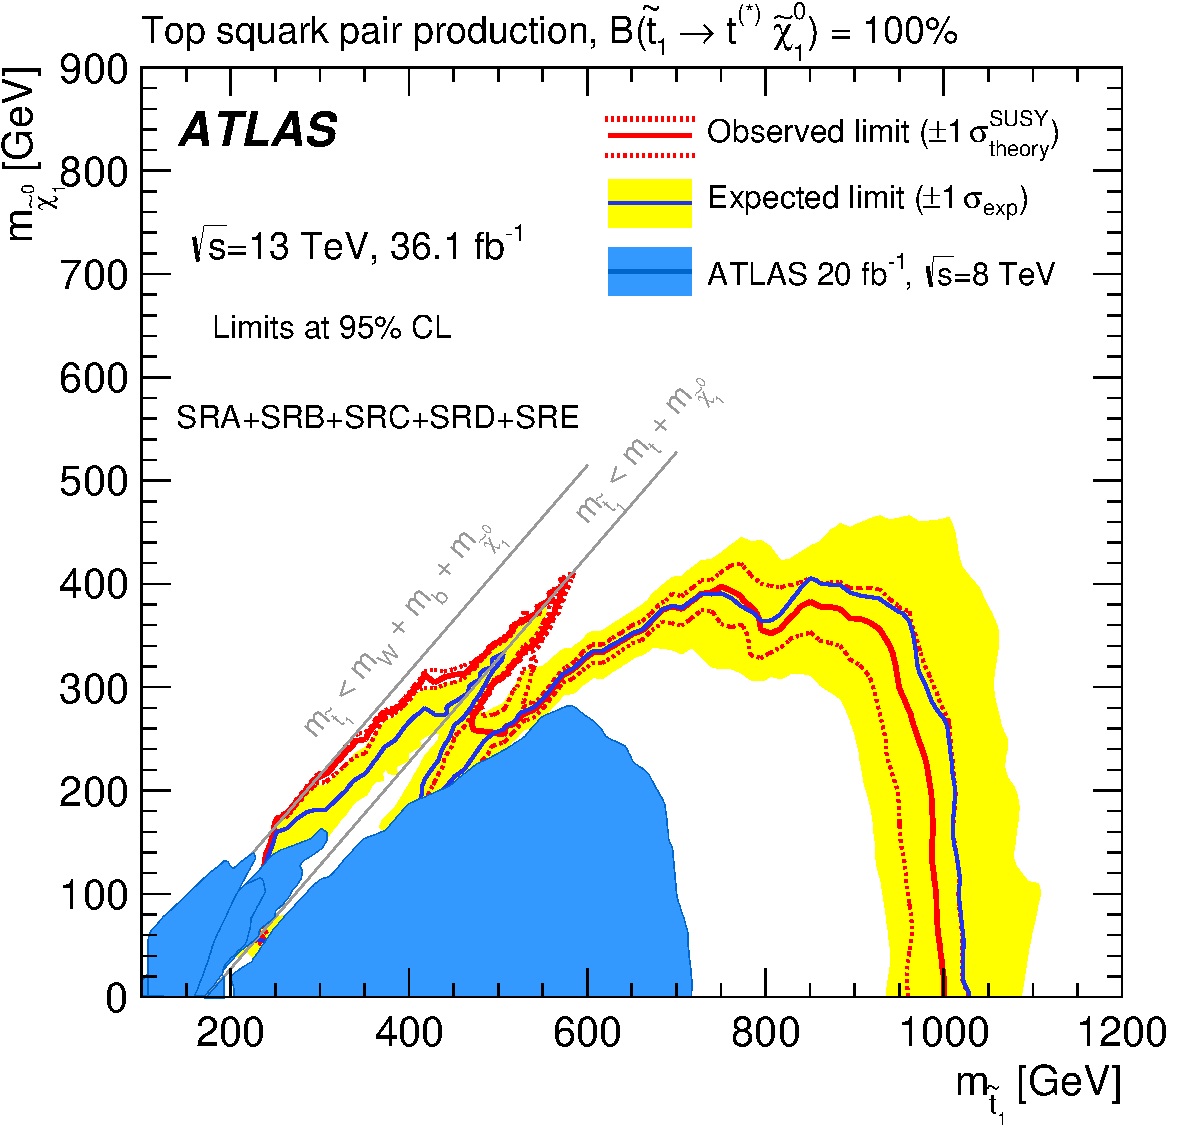
\includegraphics[width=0.85\textwidth]{stop/fit/atlascls_m0m12_wband1_showcms0_StopZL2016_SRABCDE}
			    \caption{Observed (red solid line) and expected (blue solid line)
			      exclusion contours at 95\% CL as a function of $\stop$ and
			      $\ninoone$ masses in the scenario where both top squarks decay
			      via $\stop\to t^{(*)} \ninoone$. Masses that are within the contours are excluded. Uncertainty bands corresponding to the $\pm 1
			      \sigma$ variation of the expected limit (yellow band) and the
			      sensitivity of the observed limit to $\pm 1\sigma$ variations of
			      the signal theoretical uncertainties (red dotted lines) are also
			      indicated~\cite{stop0L}. Observed limits from all third-generation Run-1 searches~\cite{Atlas8TeVSummary} at $\sqrt{s}=8$ TeV overlaid for comparison in blue (taken from~\cite{stop0L}).}
			    \label{fig:SRABC_exclusion}
			  \end{center}
			\end{figure}

			Signal models where top-squark decays into $b \chinoonepm$, or into additional massive neutralinos, are interpreted in four different scenarios~\cite{stop0L}:

			\begin{description}
			  \item[\boldmath Natural SUSY-inspired mixed grid:] this is a simplified model~\cite{Papucci2011} where $m_{\chinoonepm}=\mLSP+1\gev$ with two decay modes, $\stop\to b \chinoonepm$ and $\stop\to t\LSP$. Only on-shell top-quark decays are considered. The maximal mixing between the partners of the left- and right-handed top quarks, and the nature of the \LSP\ (pure bino) is assumed to be the same as for the $B$($\stop\to t\LSP$)=$100\%$ case. The branching ratio to $\stop\to t\LSP$ is set to $0\%$, $25\%$, $50\%$, and $75\%$. The limits obtained are shown in Figure~\ref{fig:tbMet_exclusion}~\cite{stop0L}).

				\item[\boldmath Non-asymptotic higgsino:] a simplified model inspired to the \ac{pMSSM} with a higgsino \ac{LSP}, ${m_{\chinoonepm}=\mLSP+5\gev}$, and ${m_{\ninotwo}=\mLSP+10\gev}$. This assumes three sets of branching ratios for the considered decays of $\stop\to t\ninotwo$, $\stop\to t\LSP$, $\stop\to b\chinoonepm$~\cite{Papucci2011}. In particular, a set of branching ratios with $B$($\stop\to t\ninotwo$, $\stop\to t\LSP$, $\stop\to b\chinoonepm$) = $33\%$, $33\%$, $33\%$, which is equivalent to a \ac{pMSSM} model with the lightest top squark mostly consisting of the superpartner of left-handed top quark and $\tanb=60$, is considered; and other two sets of branching ratios $B$($\stop\to t\ninotwo$, $\stop\to t\LSP$, $\stop\to b\chinoonepm$) = $45\%$, $10\%$, $45\%$ and $B$($\stop\to t\ninotwo$, $\stop\to t\LSP$, $\stop\to b\chinoonepm$) = $25\%$, $50\%$, $25\%$ are considered. These correspond to the scenarios in which $\mqlthree < \mtr$, independently of the choice of \tanb, and $\mtr<\mqlthree$ with $\tanb=20$, respectively. As mentioned in Chapter~\ref{ch:theory}, \mqlthree\ represents the left-handed third-generation mass parameter and \mtr\ is the mass parameter of the superpartner to the right-handed top quark. The limits for this interpretation are shown in Figure~\ref{fig:nonAsymhiggsino_exclusion} in the \mstop-\mLSP\ plane~\cite{stop0L}).

				\item[\boldmath Wino-NLSP pMSSM:] this is a \ac{pMSSM} model where the \ac{LSP} is bino-like with mass \mone\ and the \ac{NLSP} is wino-like with mass \mtwo, with $\mtwo=2\mone$ and $\mstop>\mone$~\cite{Papucci2011}. Limits (Figure~\ref{fig:winoNLSP_exclusion}) are set for both positive and negative higgsino mass parameter, $\mu$, as a function of the \stop\ and \ninoone\ masses which can be translated to different \mone\ and \mqlthree. In this interpretation only bottom- and top-squark production are considered. Furthermore, in this model the allowed decays in the top-squark production scenario are $\stop\to t \ninotwo\to h/Z \LSP$, with a maximum branching ratio of 33\%, and $\stop \to b \chinoonepm$. The $\ninotwo$ decay into either a $h$ or $Z$ is determined by the sign of $\mu$. In addition, the $\stop\to t\LSP$ decay with 100\% branching ratio is also considered along the diagonal region. The equivalent decays in bottom-squark production are $\sbottom\to t\chinoonepm$ and $\sbottom\to b\ninotwo$~\cite{stop0L}). %The remaining \ac{pMSSM} parameters have the following values: $\mthree=2.2$ TeV (gluino mass parameter), $\ms=\sqrt{m_{\stopone} m_{\stoptwo}}=1.2$ TeV (geometric mean of top-squark masses), $\xtms=\sqrt{6}$ (mixing parameter between the superpartners of left- and right-handed states, where $X_{t}=\at-\mu/\tanb$ and $\at$ is the trilinear coupling parameter in the top-quark sector), and $\tanb=20$. All other \ac{pMSSM} masses are set to $>3$ \TeV.

				\item[\boldmath Well-tempered neutralino pMSSM:] in this \ac{pMSSM} model three light neutralinos and a light chargino (mixtures of bino and higgsino states), are considered with masses within $50$~\GeV\ of the lightest state~\cite{atlasDM,wellTemp}. Such model is designed to satisfy the \ac{SM} Higgs boson mass and the dark-matter relic density ($0.10<\Omega h^{2}<0.12$, where $\Omega$ is energy density parameter and $h$ is the Planck constant~\cite{relic_density}).
				 %with \ac{pMSSM} parameters: $\mone=-(\mu+\delta)$ where $\delta=20$--$50\gev$, $\mtwo=2.0$ TeV, $\mthree=1.8$ TeV, $\ms=0.8$--$1.2$~\TeV, $\xtms\sim\sqrt{6}$, and $\tanb=20$. 
				The limits for this model are shown in Figure~\ref{fig:wellTemp_exclusion}. In this interpretation only bottom- and top-squark production are considered. Furthermore, the signal grid points were produced in two planes, $\mu$-\mtr\ and $\mu$-\mqlthree, and then projected to the corresponding \stop\ and \ninoone\ masse85~\cite{stop0L}).% The remaining \ac{pMSSM} masses are set to $>3$ TeV.
			\end{description}

			\begin{figure}[htpb]
			  \begin{center}
			    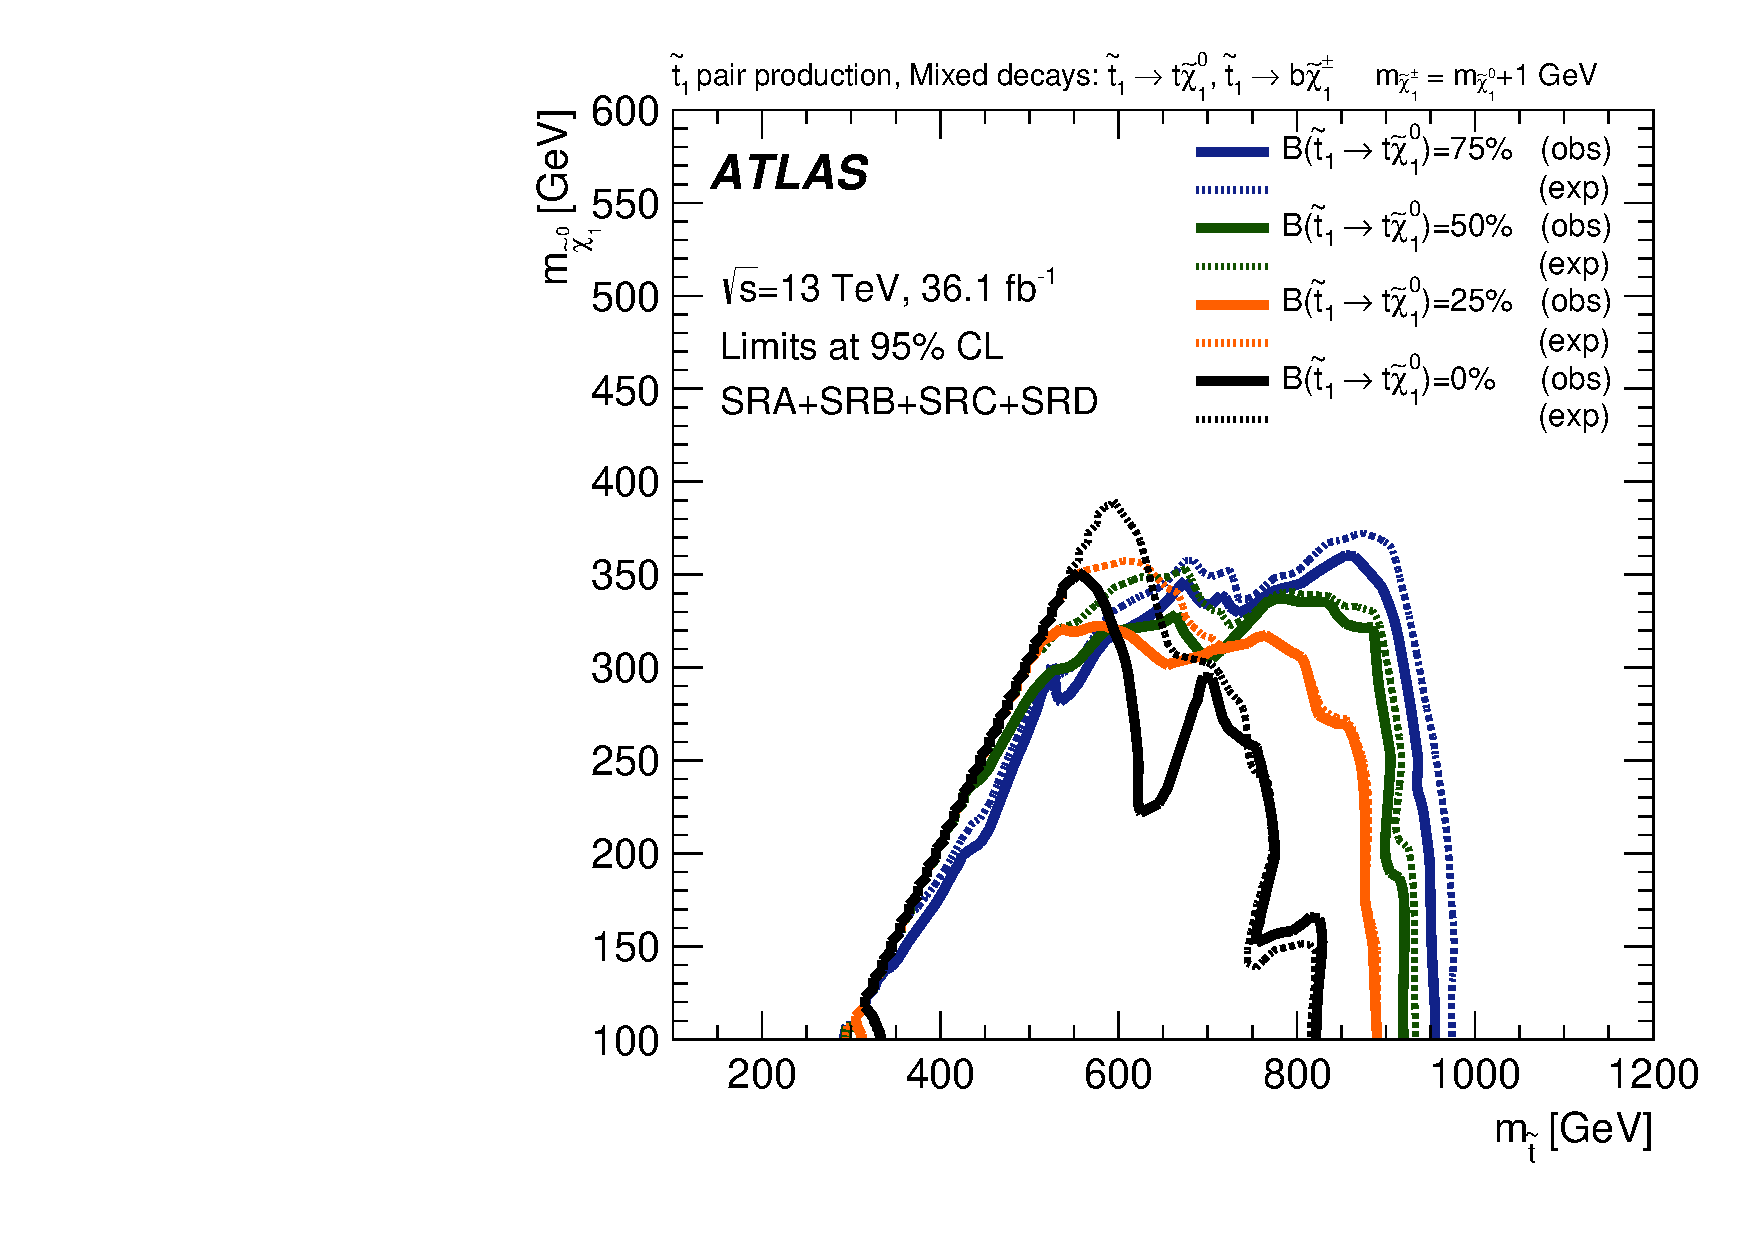
\includegraphics[width=0.85\textwidth]{figures/fit/SRABCD_mixed_dm1}
			    \caption{Observed (solid line) and expected (dashed line) exclusion contours at 95\% CL as a function of $\stop$ and $\ninoone$ masses and branching ratio to $\stop\to t\LSP$ in the natural SUSY-inspired mixed grid scenario where $m_{\chinoonepm}=\mLSP+1\gev$ (taken from~\cite{stop0L}).}
			    \label{fig:tbMet_exclusion}
			  \end{center}
			\end{figure}

			\begin{figure}[htpb]
			  \begin{center}
			   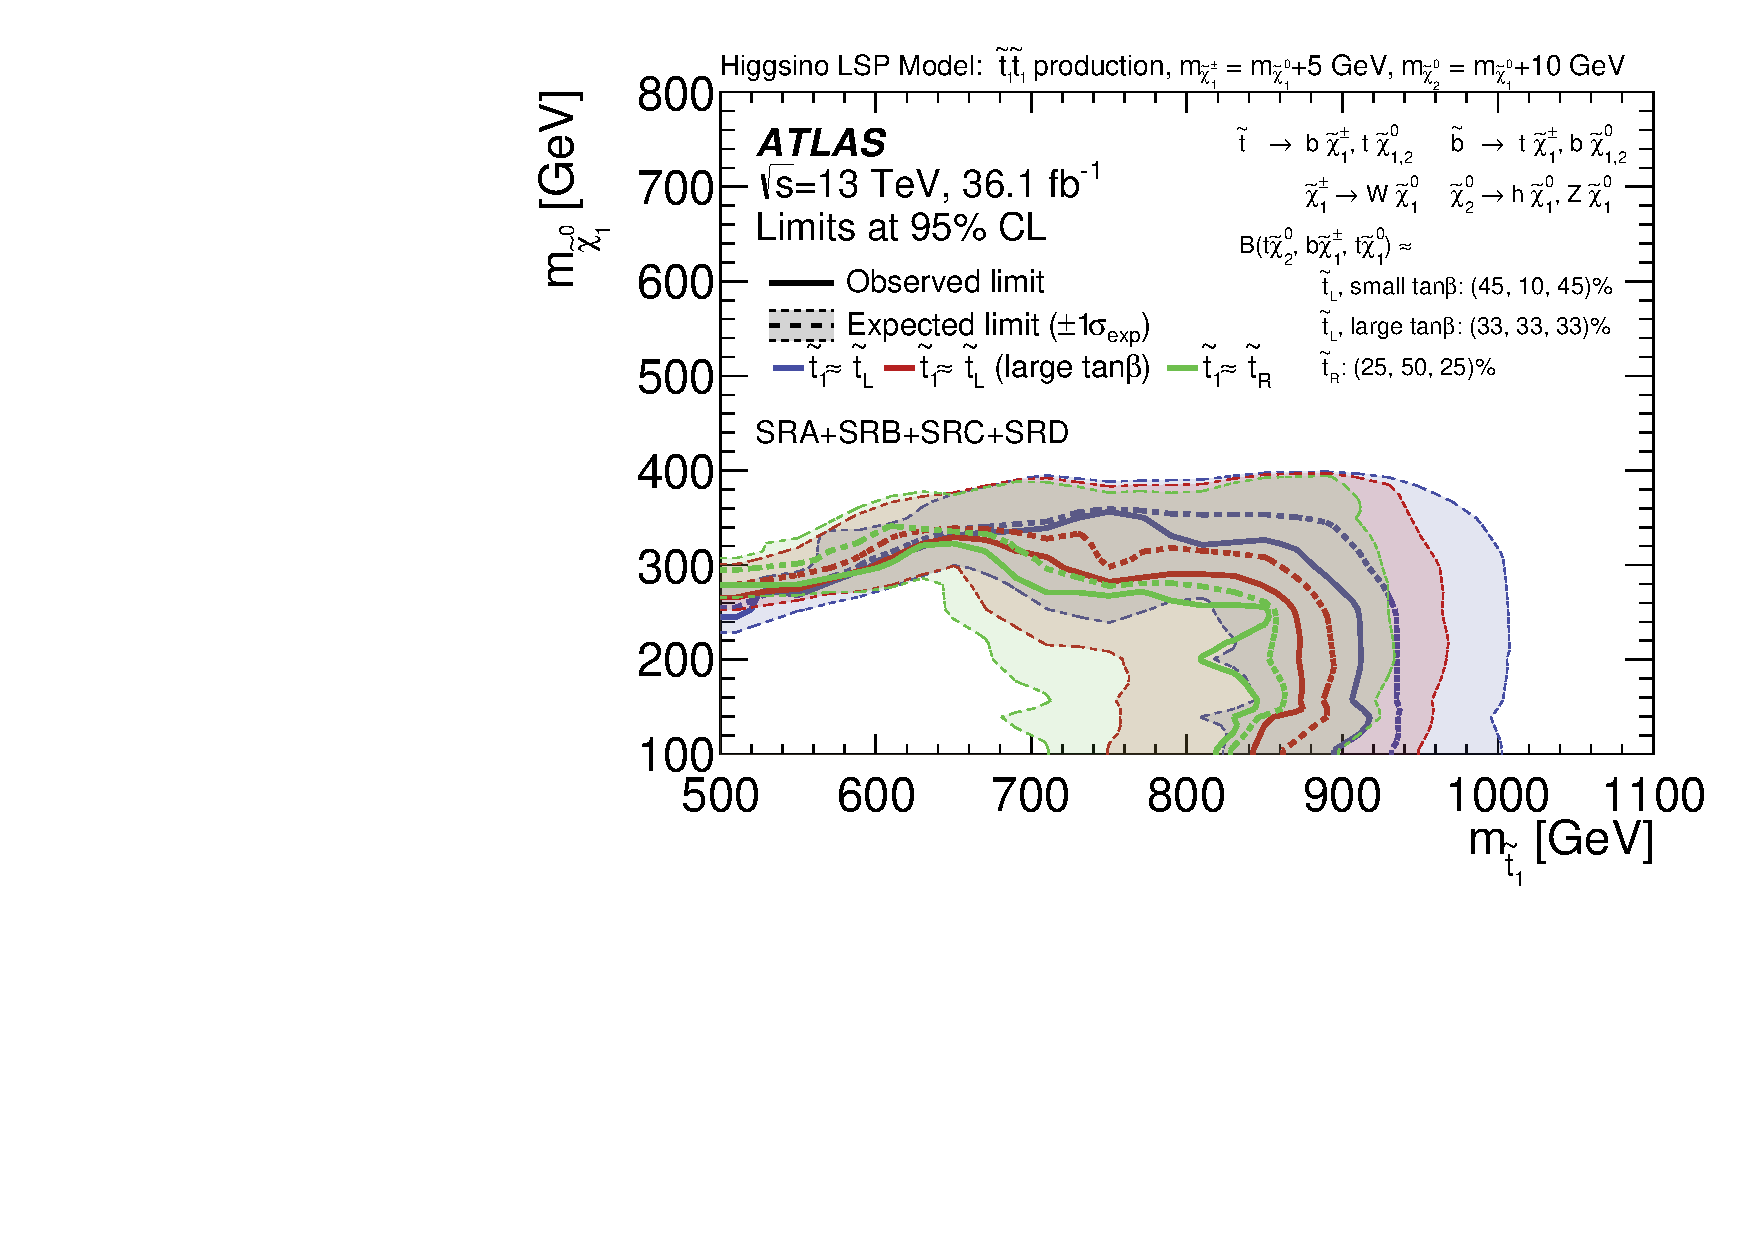
\includegraphics[width=0.85\textwidth]{figures/fit/SRABCD_tN1tN2bC1.pdf}
			    \caption{Observed (solid line) and expected (dashed line) exclusion contours at 95\% CL as a function of \mstop\ and \mLSP\ for the pMSSM-inspired non-asymptotic higgsino simplified model for a small tan$\beta$ with $B$($\stop\to t\ninotwo$, $\stop\to t\LSP$, $\stop\to b\chinoonepm$) = 45\%, 10\%, 45\% (blue), a large tan$\beta$ with $B$($\stop\to t\ninotwo$, $\stop\to t\LSP$, $\stop\to b\chinoonepm$) = 33\%, 33\%, 33\% (red), and a small $\tilde t_{R}$ with $B$($\stop\to t\ninotwo$, $\stop\to t\LSP$, $\stop\to b\chinoonepm$) = 25\%, 50\%, 25\% (green) assumption. Uncertainty bands correspond to the $\pm 1 \sigma$ variation of the expected limit(taken from~\cite{stop0L}).}
			    \label{fig:nonAsymhiggsino_exclusion}
			  \end{center}
			\end{figure}

			\begin{figure}[htpb]
			  \begin{center}
			    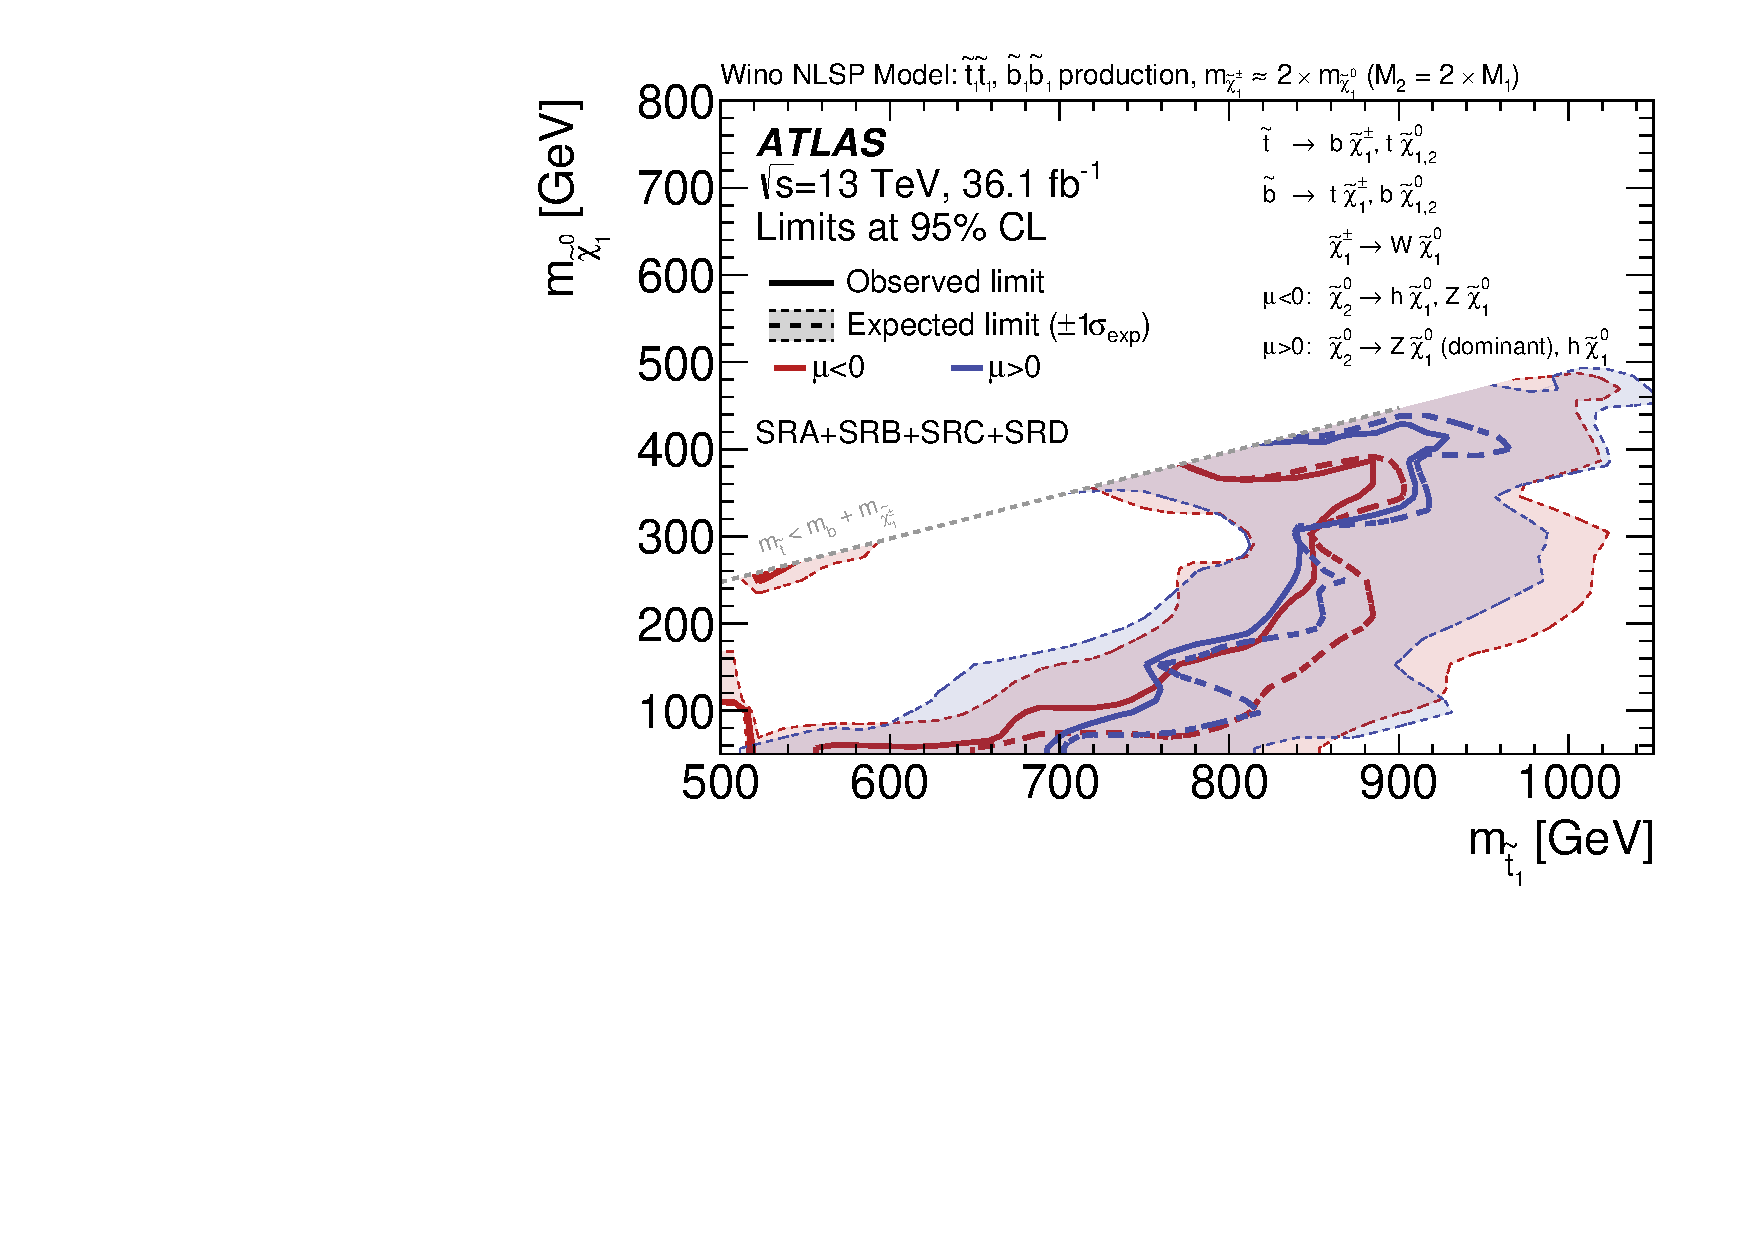
\includegraphics[width=0.85\textwidth]{figures/fit/SRABCD_winoNLSP.pdf}
			    \caption{Observed (solid line) and expected (dashed line) exclusion contours at 95\% CL as a function of $\stop$ and $\ninoone$ masses for the Wino NLSP pMSSM model for both positive (blue) and negative (red) values of $\mu$. Uncertainty bands correspond to the $\pm 1 \sigma$ variation of the expected limit (taken from~\cite{stop0L}).}
			    \label{fig:winoNLSP_exclusion}
			  \end{center}
			\end{figure}

			\begin{figure}[htpb]
			  \begin{center}
			    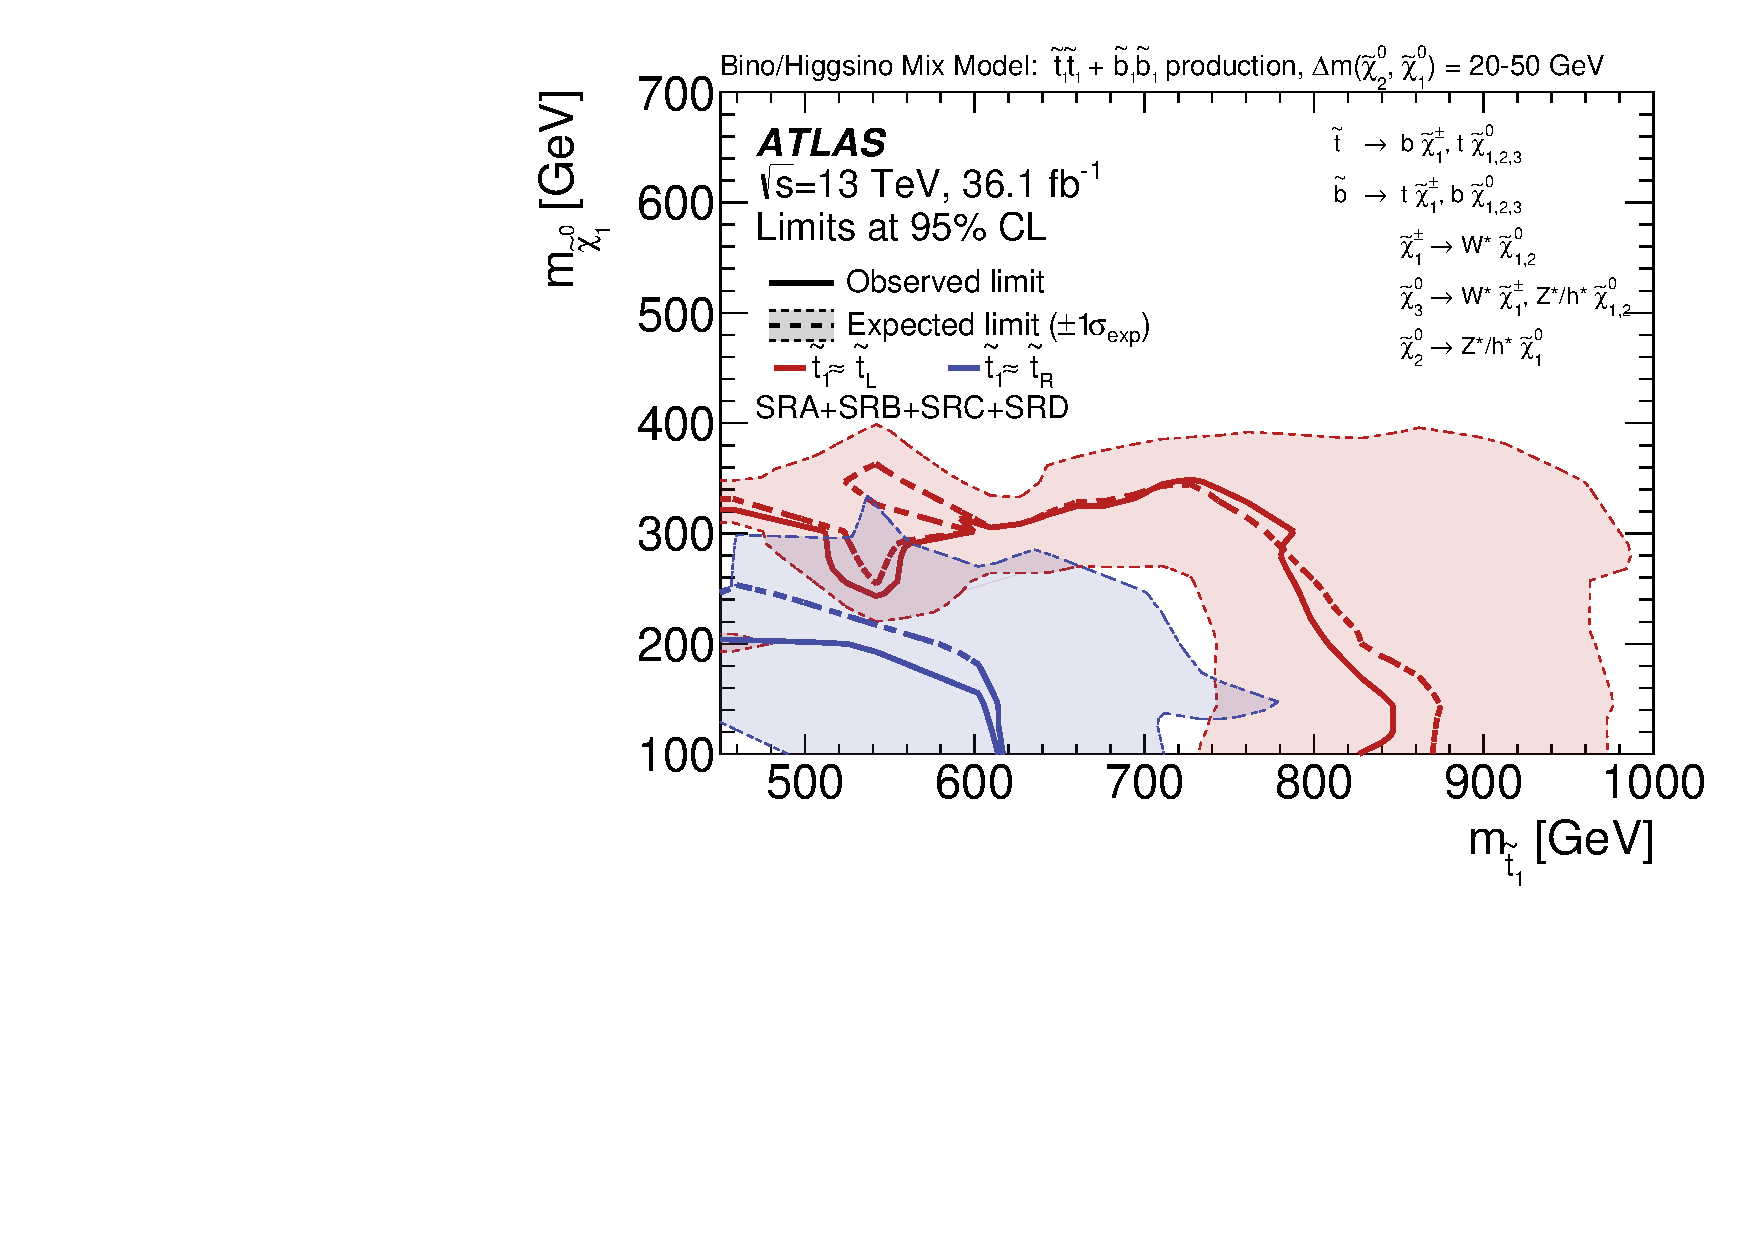
\includegraphics[width=0.85\textwidth]{figures/fit/SRABCD_wellTempered.pdf}
			    \caption{Observed (solid line) and expected (dashed line) exclusion contours at 95\% CL as a function of $\stop$ and $\ninoone$ masses for the $\tilde t_{L}$ scan (red) as well as for the $\tilde t_{R}$ scan (blue) in the well-tempered pMSSM model. Uncertainty bands correspond to the $\pm 1 \sigma$ variation of the expected limit (taken from~\cite{stop0L}).} 
			    \label{fig:wellTemp_exclusion}
			  \end{center}
			\end{figure}

			Finally, the results for SRE are interpreted for gluino-mediated top-squark production via gluino decays in terms of the \stop-$\gluino$ mass plane with $\Delta m(\stop,\ninoone)=5\GeV$. Figure~\ref{fig:SRE_exclusion} shows the exclusion plot of gluino masses up to $m_{\gluino}=1800\GeV$ with $\mstop<800\GeV$~\cite{stop0L}).

			\begin{figure}[htpb]
			  \begin{center}
			    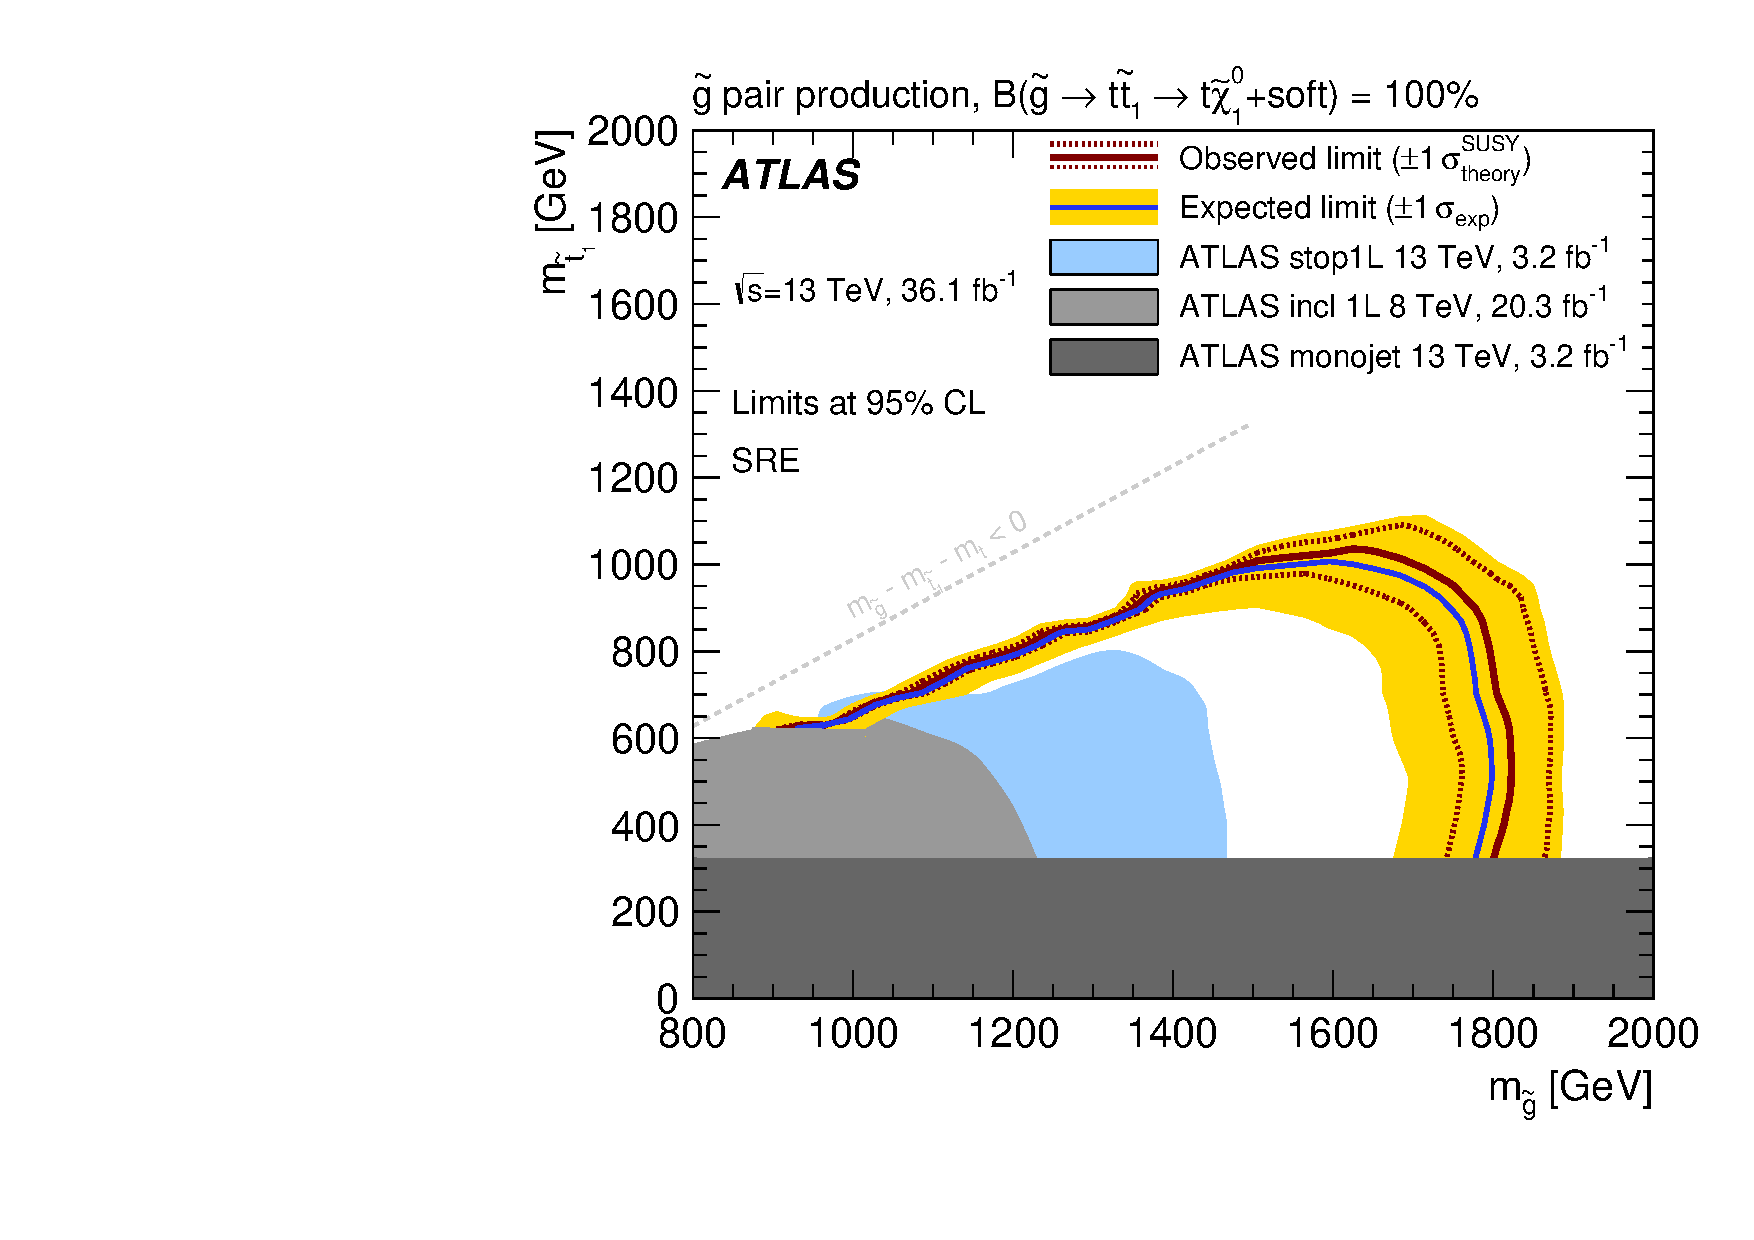
\includegraphics[width=0.85\textwidth]{figures/fit/SRE_exclusion}
			    \caption{Observed (red solid line) and expected (blue solid line)
			      exclusion contours at 95\% CL as a function
			      of $\gluino$ and $\stop$ masses in the scenario where both
			      gluinos decay via $\gluino\to t\stop\to t\ninoone+$soft
			      and $\Delta m(\stop,\ninoone)=5\GeV$. Uncertainty bands corresponding to the $\pm 1
			      \sigma$ variation of the expected limit (yellow band) and the
			      sensitivity of the observed limit to $\pm 1\sigma$ variations of
			      the signal theoretical uncertainties (red dotted lines) are also
			      indicated. Observed limits from previous searches with the ATLAS detector at $\sqrt{s}=8$ and $\sqrt{s}=13$ TeV are overlaid in grey and blue~\cite{stop1L,Gtc1L,GtcMonojet} (taken from~\cite{stop0L}).}
			    \label{fig:SRE_exclusion}
			  \end{center}
			\end{figure}
